\chapter{Results}
The three path planners (HV, $N$-HV, and MCPP) introduced in Chapter \ref{ch:pp} all aim to reduce the overall prediction uncertainty of a field given a limited amount of flight time. They accomplish the task by calculating variances of a target field's predictions and attempting to choose a trajectory that reduces overall uncertainty. 

The number of trajectories compared in both the $N$-HV and MCPP methods is $N=5$. For the MCPP method, an additional $M_{mc}=10$ Monte Carlo trajectories are calculated for each of the $N$ trajectories. The target field size of the fields compared in the simulation have unit-less vesicle dimensions of $100\times 100$. Two random number generator seeds ($2$, $3$) are used to generate two sets of runs in an effort to show the methods for a variety of random fields. The autocorrelation factors of the field will be varied in an effort to show the effectiveness of the methods for different field statistics. When the prediction errors and variances of the methods are compared, the values are normalized to an a priori mean variance, which is equal to the mean error and variance of the field generated from running a Kriging prediction on the equivalent field from a set of ten samples taken from the main diagonal vesicles of the target field.

\section{Prediction Error Calculation}
The quality of each path planner will be judged by its ability to explore a field with a fixed exploration path length. The prediction error of each method will be used as a criterion of path planning quality.

The prediction error function, $E (Z,\hat{Z})$, will be the average root mean square (RMS) error for all $N\times N$ points on the actual field, $Z$, and the predicted field, $\hat{Z}$.

\begin{equation}
E (Z, \hat{Z}) = \frac{1}{N^2}\sum_{\forall \vect{s}_i \in Z} (Z(\vect{s}_i) - \hat{Z}(\vect{s}_i))^2
\end{equation}

\section{High Spatial Autocorrelation Results}
The methods will be compared on target fields generated with an autocorrelation factor, $\sigma_{field}$, equal to the field width.

\begin{figure}[htb!]
    \centering
    \begin{subfigure}[t]{0.25\textwidth}
        \centering
        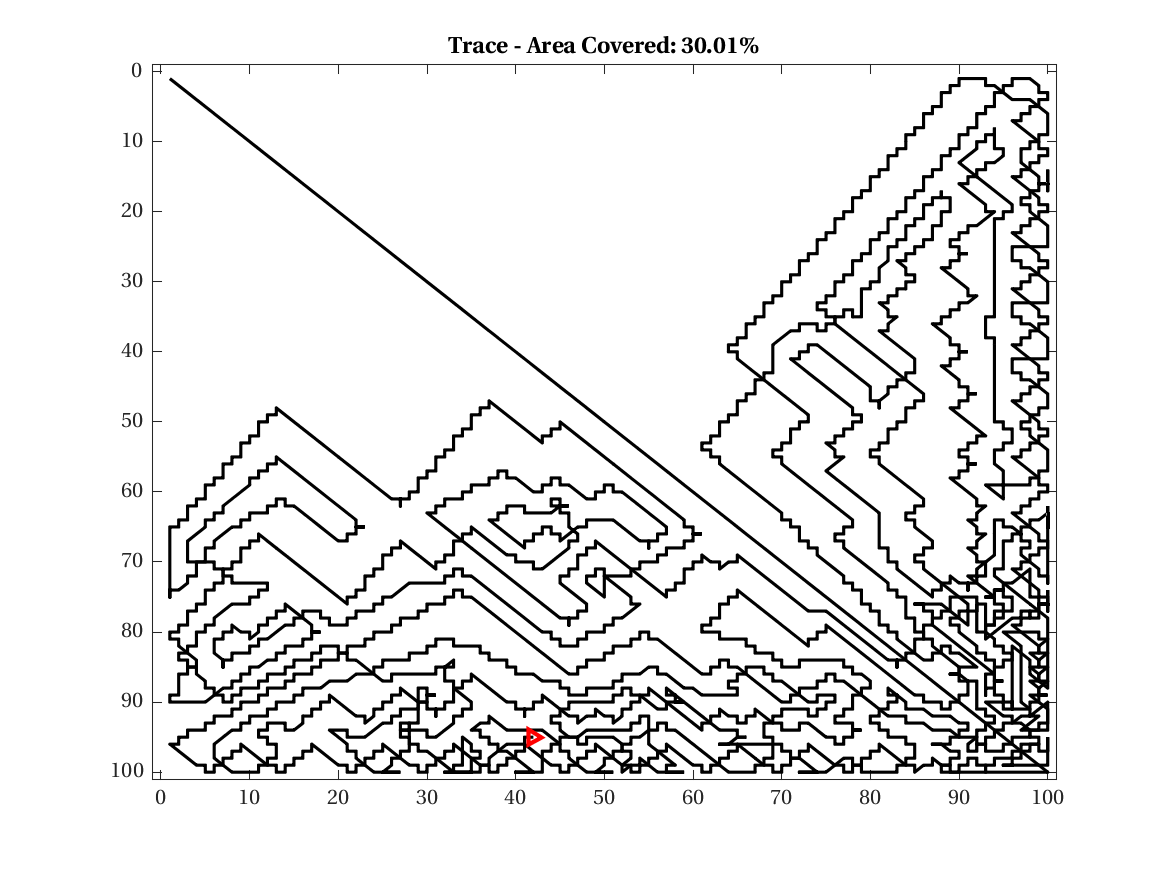
\includegraphics[width=\linewidth]{figures/path_greedy_30p_100x100_sf_100_seed_1.png}
        \captionsetup{skip=0.20\baselineskip,size=footnotesize}
        \caption{Greedy NBV}
    \end{subfigure}%
    \begin{subfigure}[t]{0.25\textwidth}
        \centering
        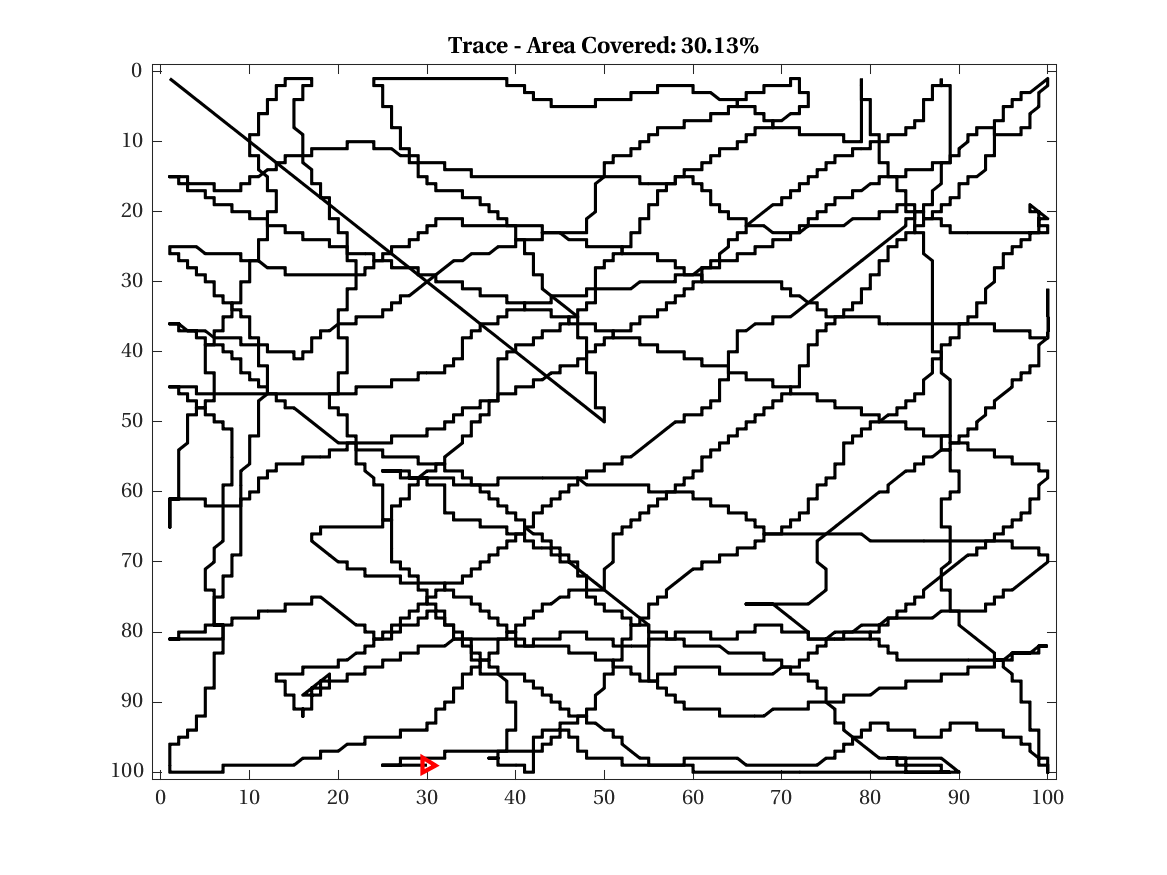
\includegraphics[width=\linewidth]{figures/path_mc_30p_100x100_sf_100_seed_1.png}
        \captionsetup{skip=0.20\baselineskip,size=footnotesize}
        \caption{MCPP}
    \end{subfigure}%
    \begin{subfigure}[t]{0.25\textwidth}
        \centering
        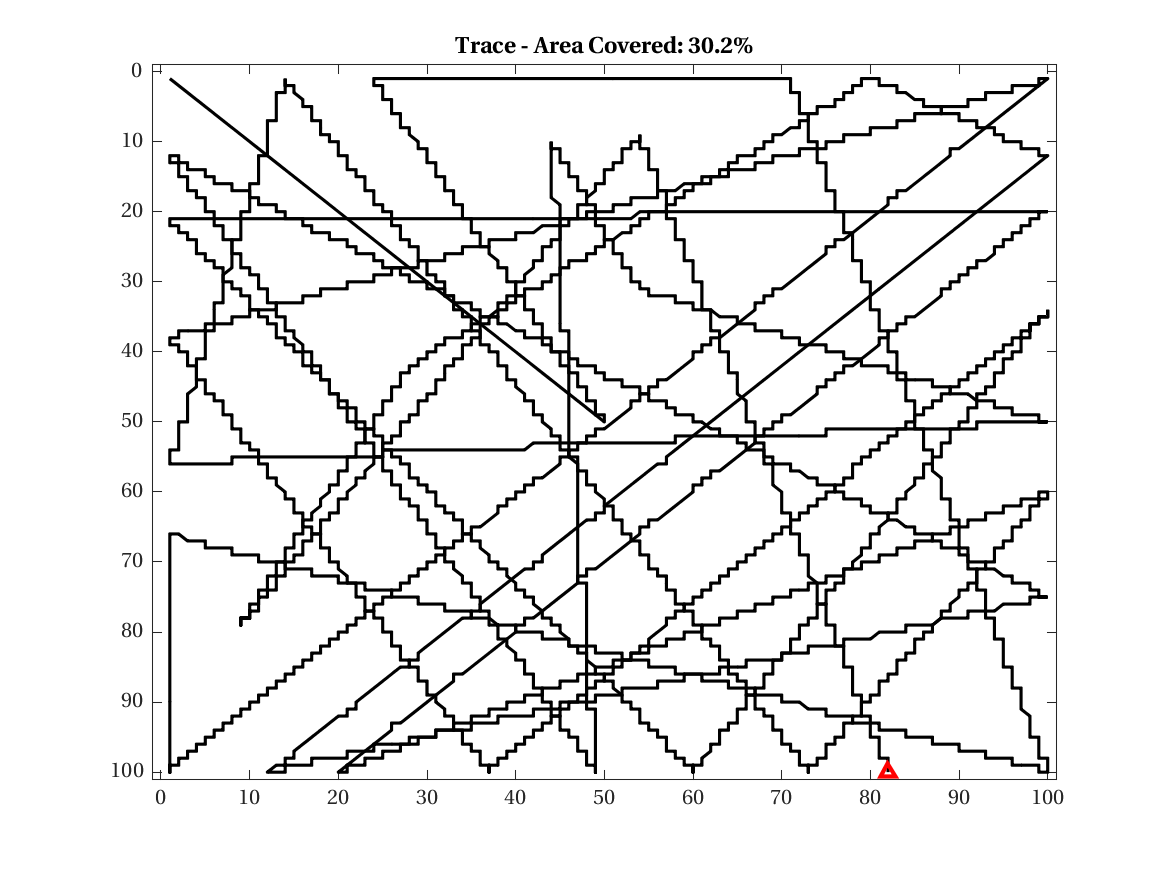
\includegraphics[width=\linewidth]{figures/path_nhv_30p_100x100_sf_100_seed_1.png}
        \captionsetup{skip=0.20\baselineskip,size=footnotesize}
        \caption{HV}
    \end{subfigure}%
    \begin{subfigure}[t]{0.25\textwidth}
        \centering
        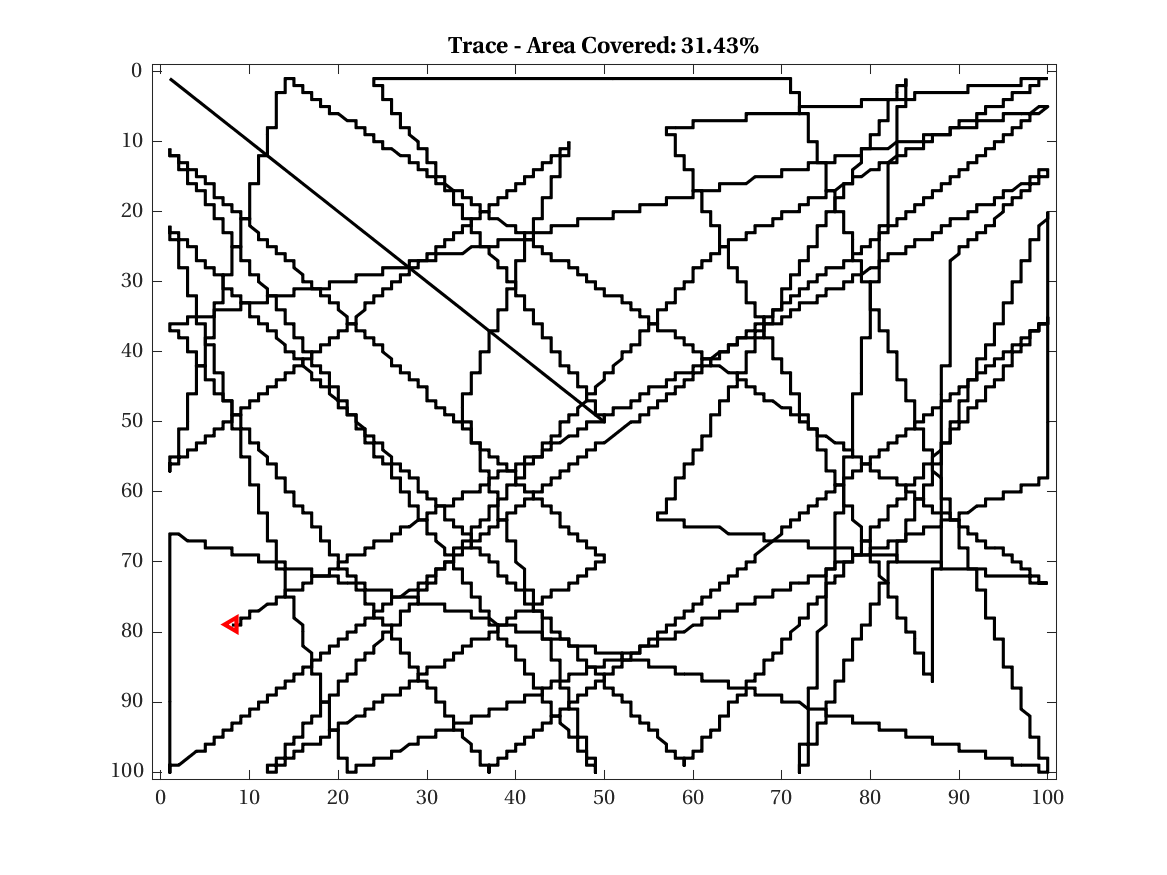
\includegraphics[width=\linewidth]{figures/path_nnhv_30p_100x100_sf_100_seed_1.png}
        \captionsetup{skip=0.20\baselineskip,size=footnotesize}
        \caption{$N$-HV}
    \end{subfigure}%
    \\
    \begin{subfigure}[t]{0.25\textwidth}
        \centering
        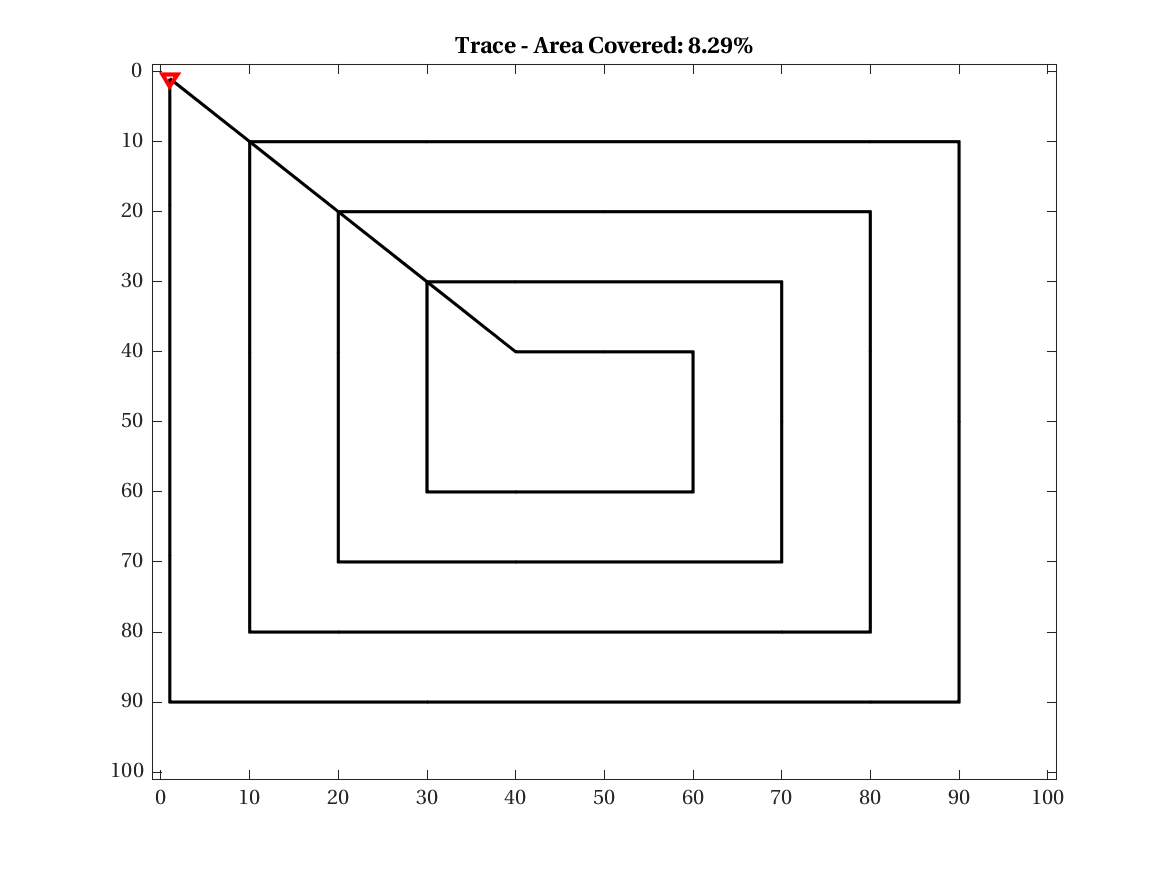
\includegraphics[width=\linewidth]{figures/path_zz_10p_100x100_sf_100_seed_1.png}
        \captionsetup{skip=0.20\baselineskip,size=footnotesize}
        \caption{$ZZ_{10}$}
    \end{subfigure}%
    \begin{subfigure}[t]{0.25\textwidth}
        \centering
        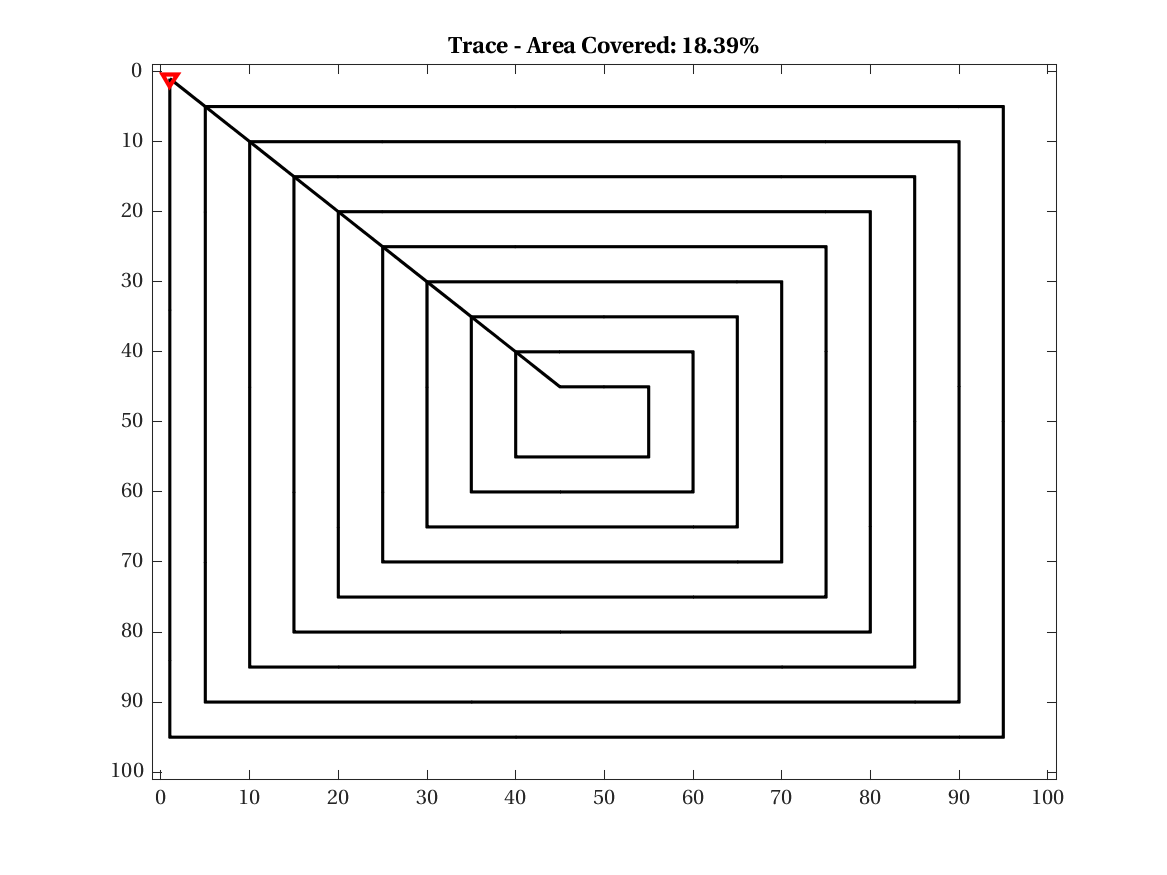
\includegraphics[width=\linewidth]{figures/path_zz_20p_100x100_sf_100_seed_1.png}
        \captionsetup{skip=0.20\baselineskip,size=footnotesize}
        \caption{$ZZ_{20}$}
    \end{subfigure}%
    \begin{subfigure}[t]{0.25\textwidth}
        \centering
        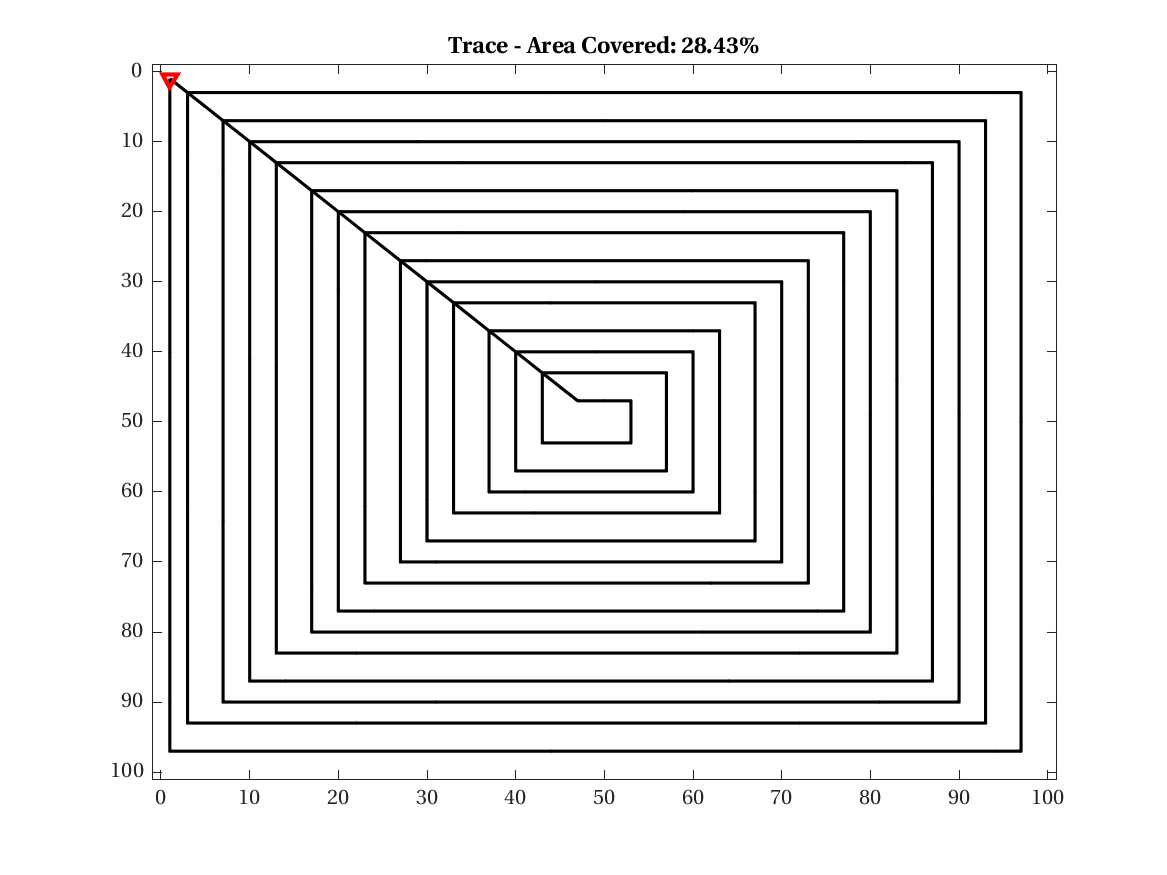
\includegraphics[width=\linewidth]{figures/path_zz_30p_100x100_sf_100_seed_1.png}
        \captionsetup{skip=0.20\baselineskip,size=footnotesize}
        \caption{$ZZ_{30}$}
    \end{subfigure}%
    \captionsetup{skip=0.20\baselineskip}
    \caption{Exploration of a field of size $100 \times 100$, $\sigma_{field} = 100$, random seed 1.}
    \label{fig:sf100}
\end{figure}

\begin{figure}[htb!]
    \centering
    \begin{subfigure}[t]{0.75\textwidth}
        \centering
        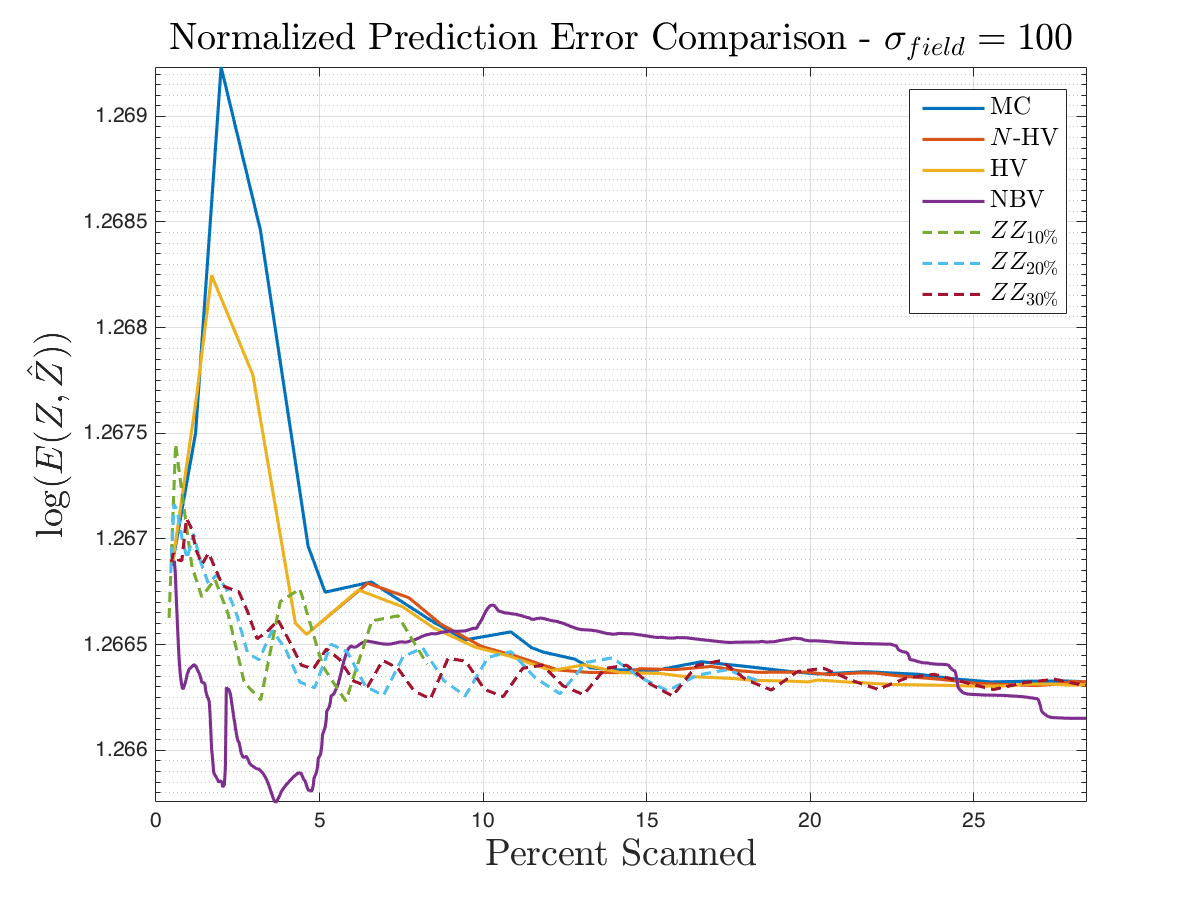
\includegraphics[width=\linewidth]{figures/normalized_errors_30p_100x100_sf_100_seed_1_app_10}
        \captionsetup{skip=0.20\baselineskip,size=footnotesize}
        \caption{Normalized prediction errors for each method.}
    \end{subfigure}%
    \\
    \begin{subfigure}[t]{0.75\textwidth}
        \centering
        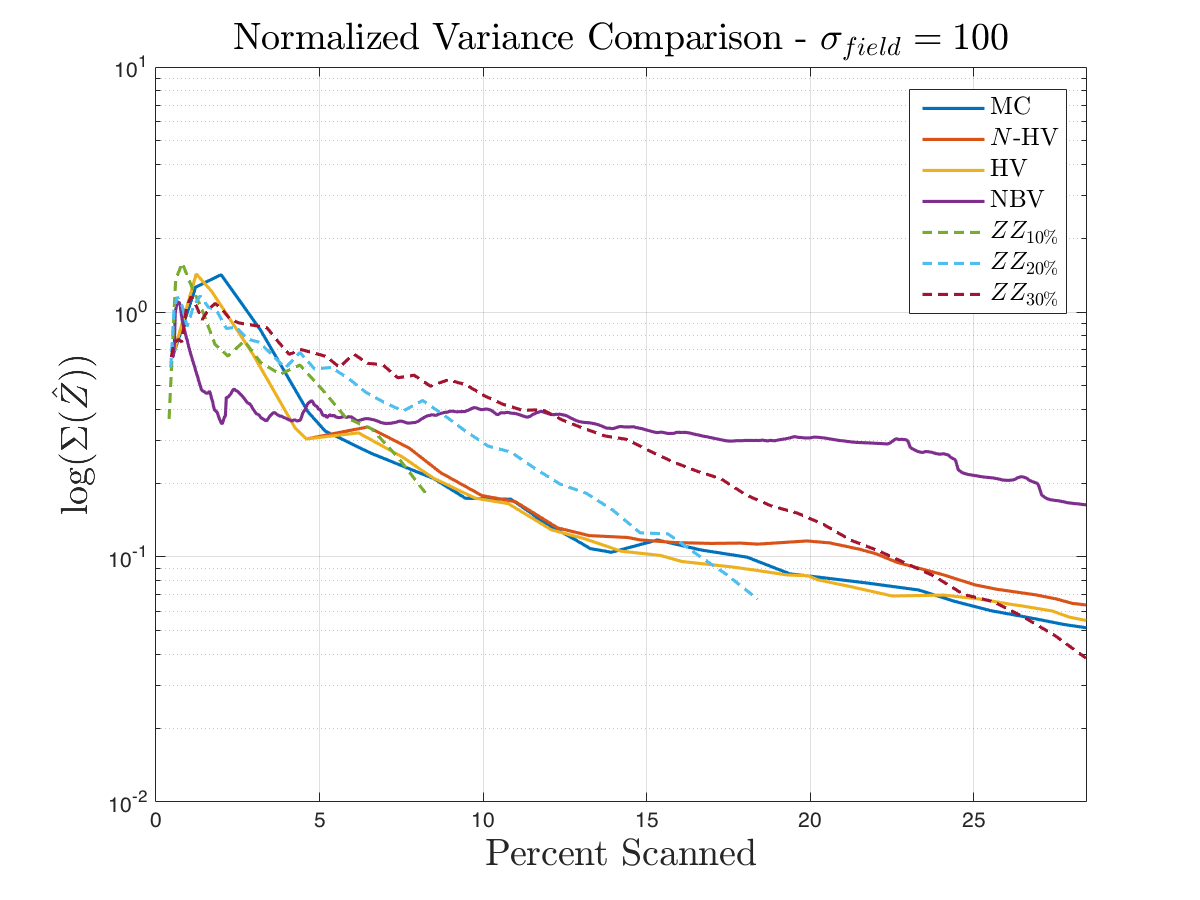
\includegraphics[width=\linewidth]{figures/normalized_variances_30p_100x100_sf_100_seed_1_app_10}
        \captionsetup{skip=0.20\baselineskip,size=footnotesize}
        \caption{Normalized prediction variances for each method.}
    \end{subfigure}%
    \captionsetup{skip=0.20\baselineskip}
    \caption{Prediction error and variances for an exploration of a field of size $100 \times 100$, $\sigma_{field} = 100$, random seed 1.}
    \label{fig:errvar100}
\end{figure}

\FloatBarrier
\clearpage\

\section{Half Width Spatial Autocorrelation Results}
The methods will be compared on target fields generated with an autocorrelation factor, $\sigma_{field}$, that is half of the field width.
\begin{figure}[htb!]
    \centering
    \begin{subfigure}[t]{0.25\textwidth}
        \centering
        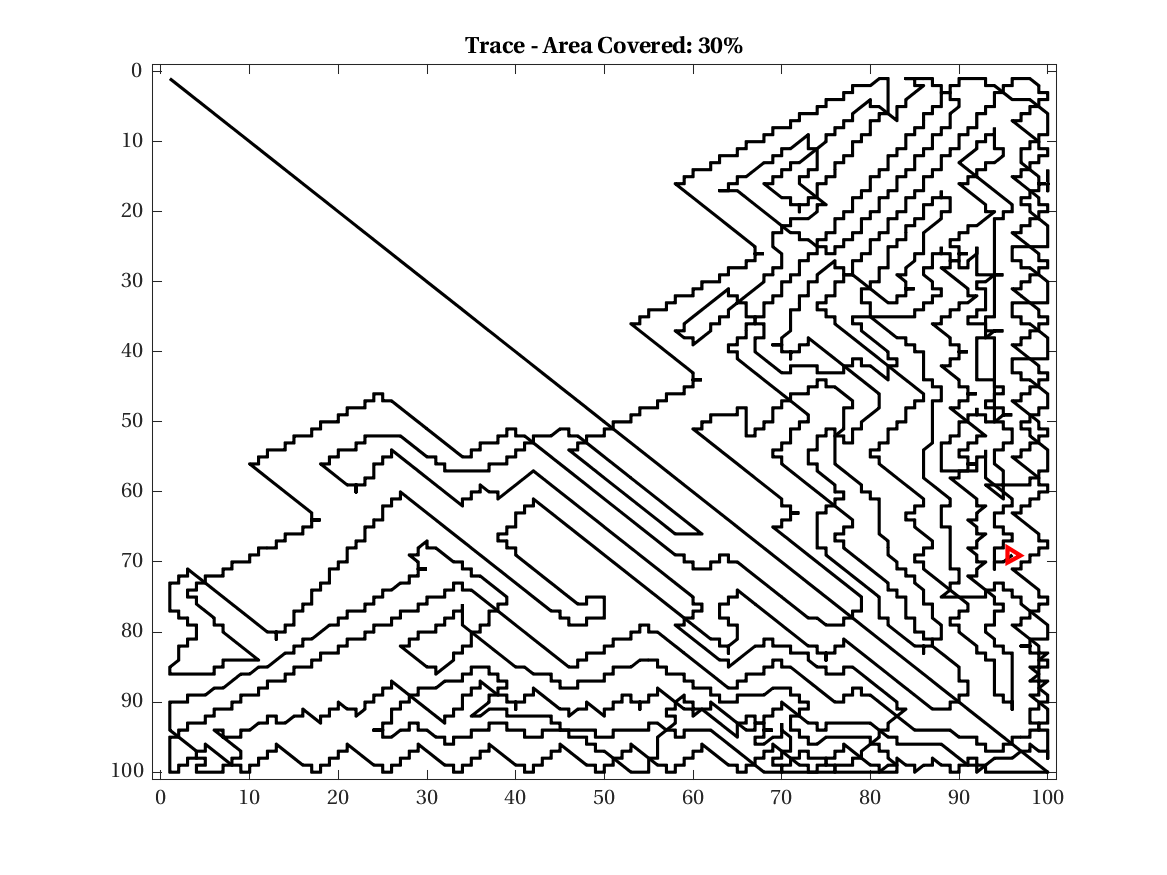
\includegraphics[width=\linewidth]{figures/path_greedy_30p_100x100_sf_50_seed_1.png}
        \captionsetup{skip=0.20\baselineskip,size=footnotesize}
        \caption{Greedy NBV}
    \end{subfigure}%
    \begin{subfigure}[t]{0.25\textwidth}
        \centering
        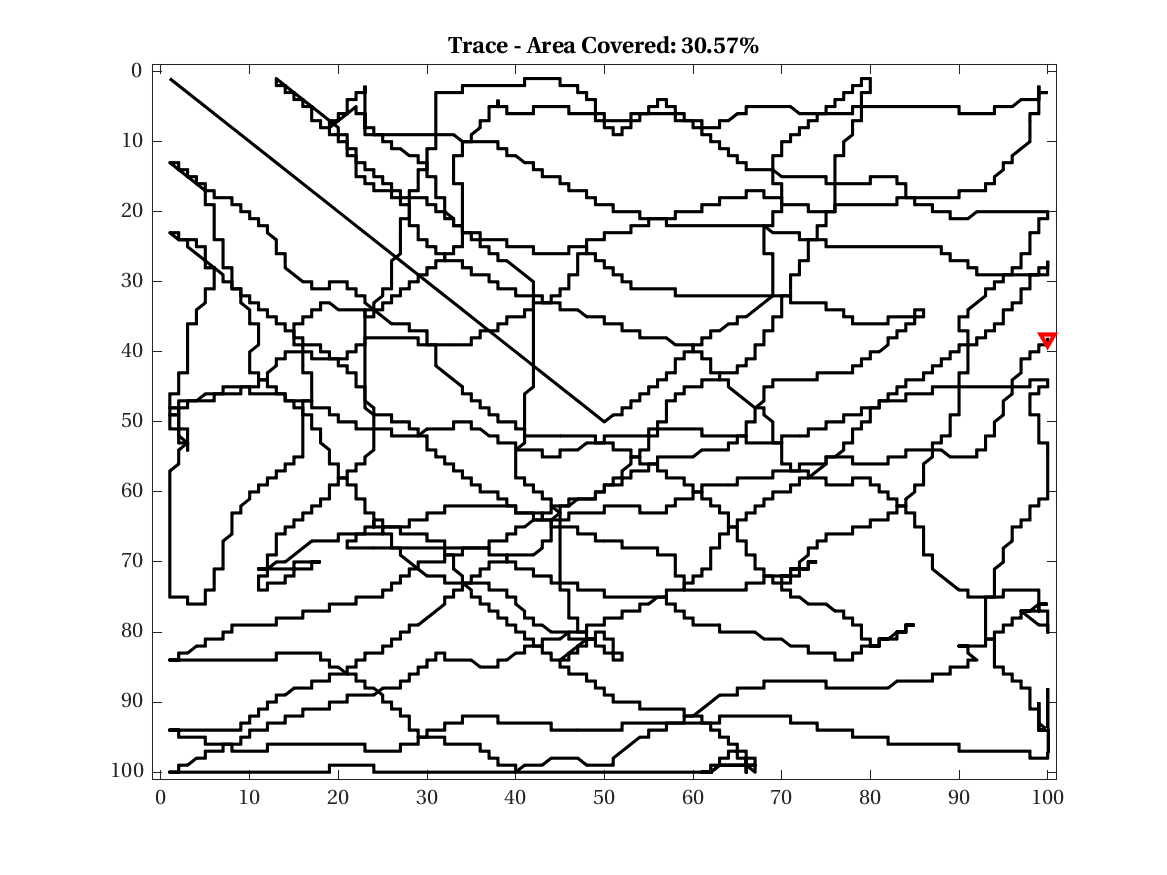
\includegraphics[width=\linewidth]{figures/path_mc_30p_100x100_sf_50_seed_1.png}
        \captionsetup{skip=0.20\baselineskip,size=footnotesize}
        \caption{MCPP}
    \end{subfigure}%
    \begin{subfigure}[t]{0.25\textwidth}
        \centering
        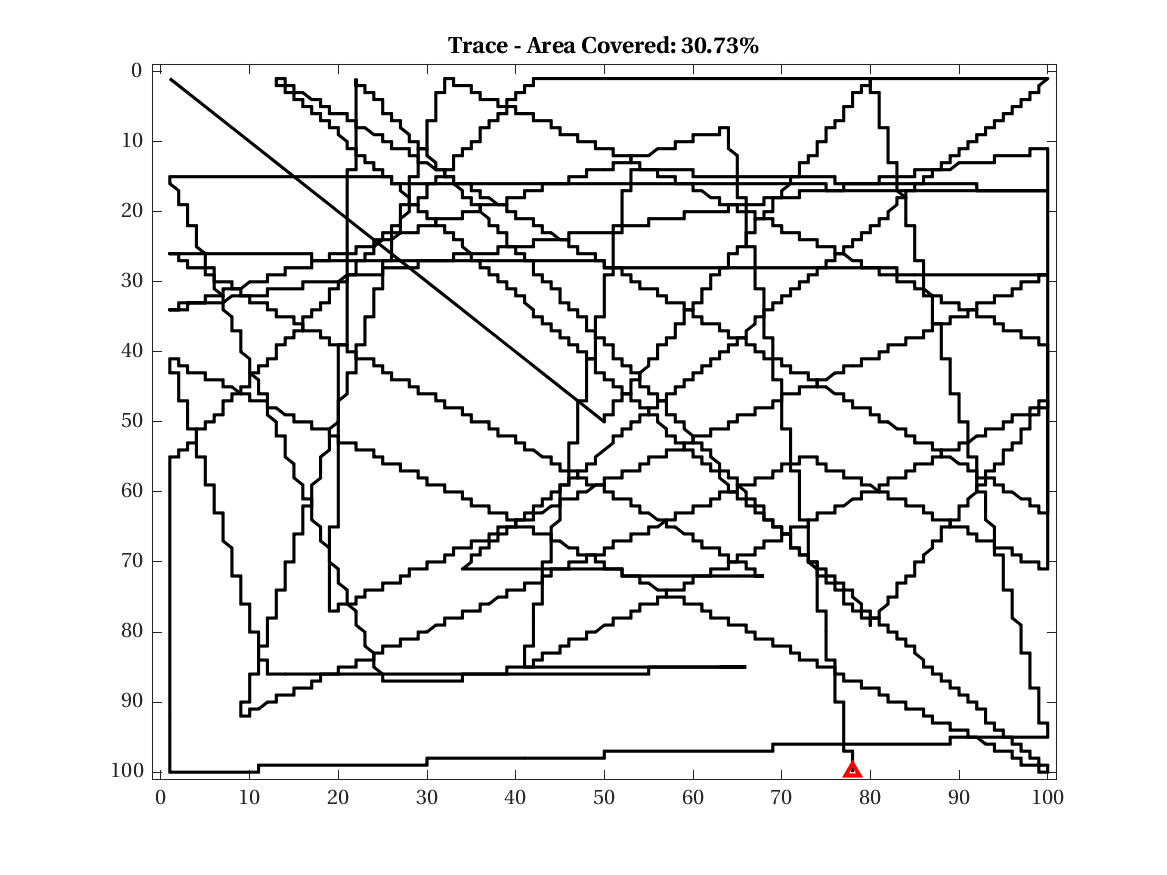
\includegraphics[width=\linewidth]{figures/path_nhv_30p_100x100_sf_50_seed_1.png}
        \captionsetup{skip=0.20\baselineskip,size=footnotesize}
        \caption{HV}
    \end{subfigure}%
    \begin{subfigure}[t]{0.25\textwidth}
        \centering
        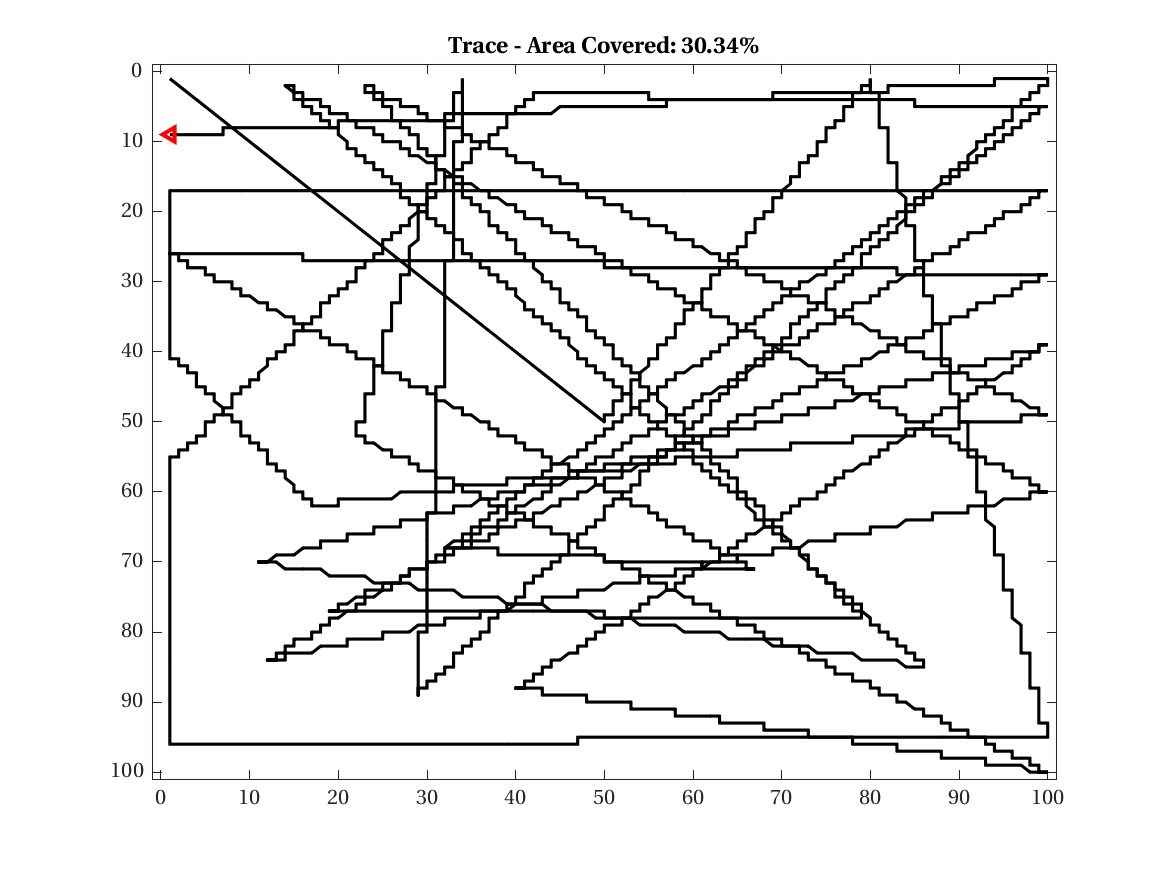
\includegraphics[width=\linewidth]{figures/path_nnhv_30p_100x100_sf_50_seed_1.png}
        \captionsetup{skip=0.20\baselineskip,size=footnotesize}
        \caption{$N$-HV}
    \end{subfigure}%
    \\
    \begin{subfigure}[t]{0.25\textwidth}
        \centering
        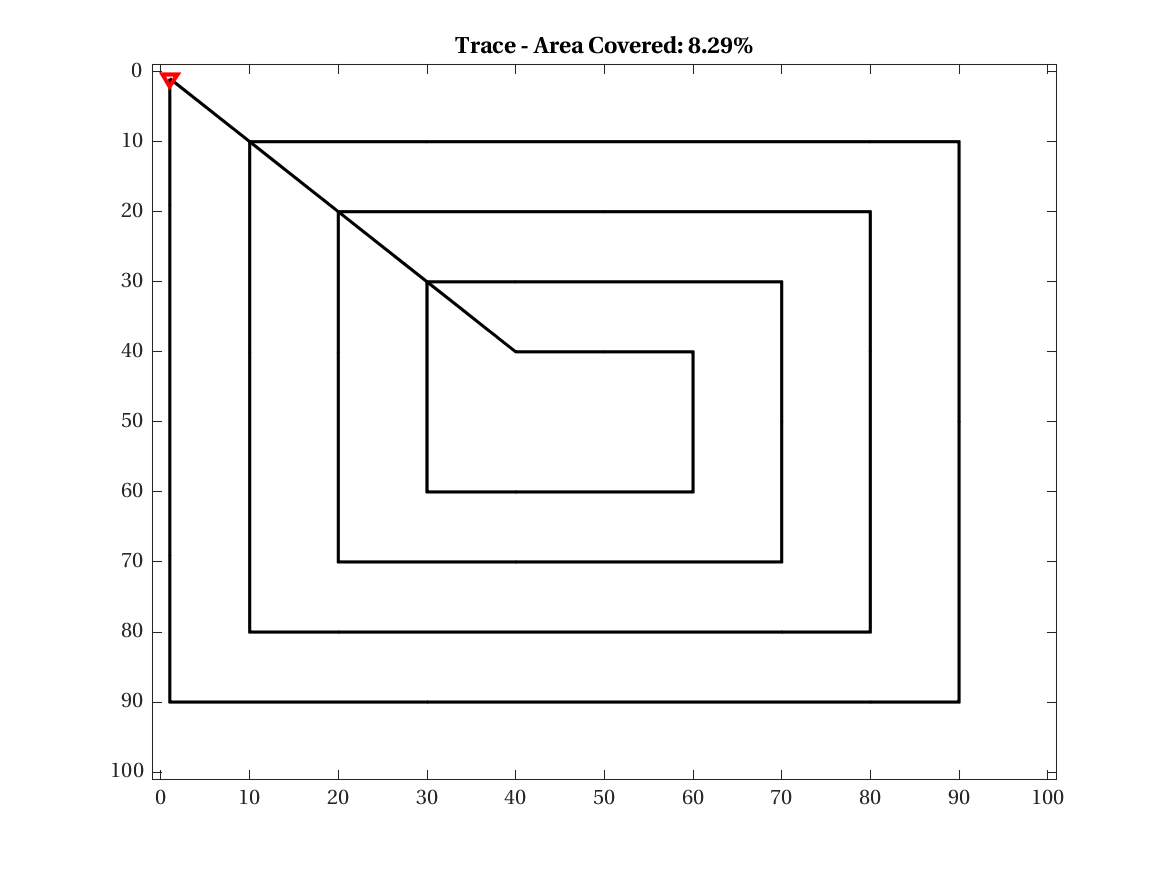
\includegraphics[width=\linewidth]{figures/path_zz_10p_100x100_sf_50_seed_1.png}
        \captionsetup{skip=0.20\baselineskip,size=footnotesize}
        \caption{$ZZ_{10}$}
    \end{subfigure}%
    \begin{subfigure}[t]{0.25\textwidth}
        \centering
        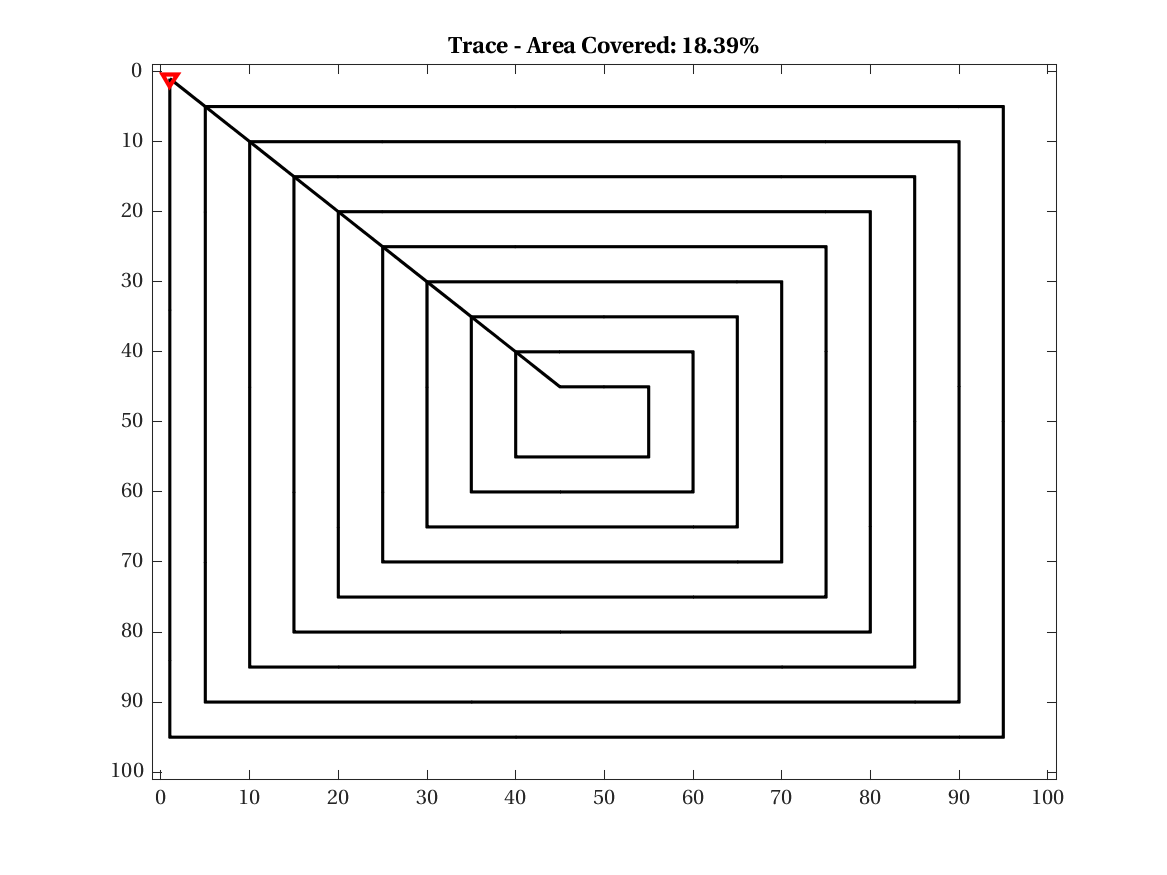
\includegraphics[width=\linewidth]{figures/path_zz_20p_100x100_sf_50_seed_1.png}
        \captionsetup{skip=0.20\baselineskip,size=footnotesize}
        \caption{$ZZ_{20}$}
    \end{subfigure}%
    \begin{subfigure}[t]{0.25\textwidth}
        \centering
        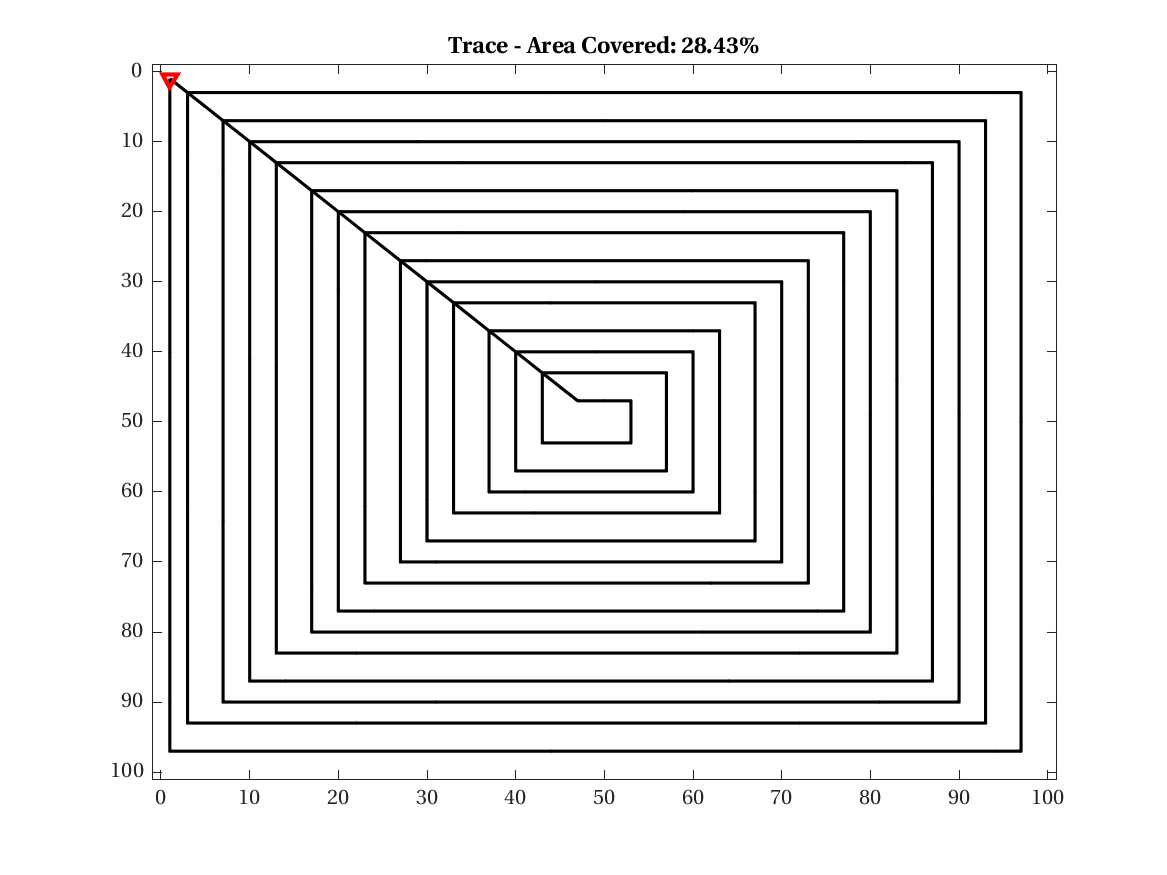
\includegraphics[width=\linewidth]{figures/path_zz_30p_100x100_sf_50_seed_1.png}
        \captionsetup{skip=0.20\baselineskip,size=footnotesize}
        \caption{$ZZ_{30}$}
    \end{subfigure}%
    \captionsetup{skip=0.20\baselineskip}
    \caption{Exploration of a field of size $100 \times 100$, $\sigma_{field} = 50$, random seed 1.}
    \label{fig:sf50}
\end{figure}

\begin{figure}[htb!]
    \centering
    \begin{subfigure}[t]{0.75\textwidth}
        \centering
        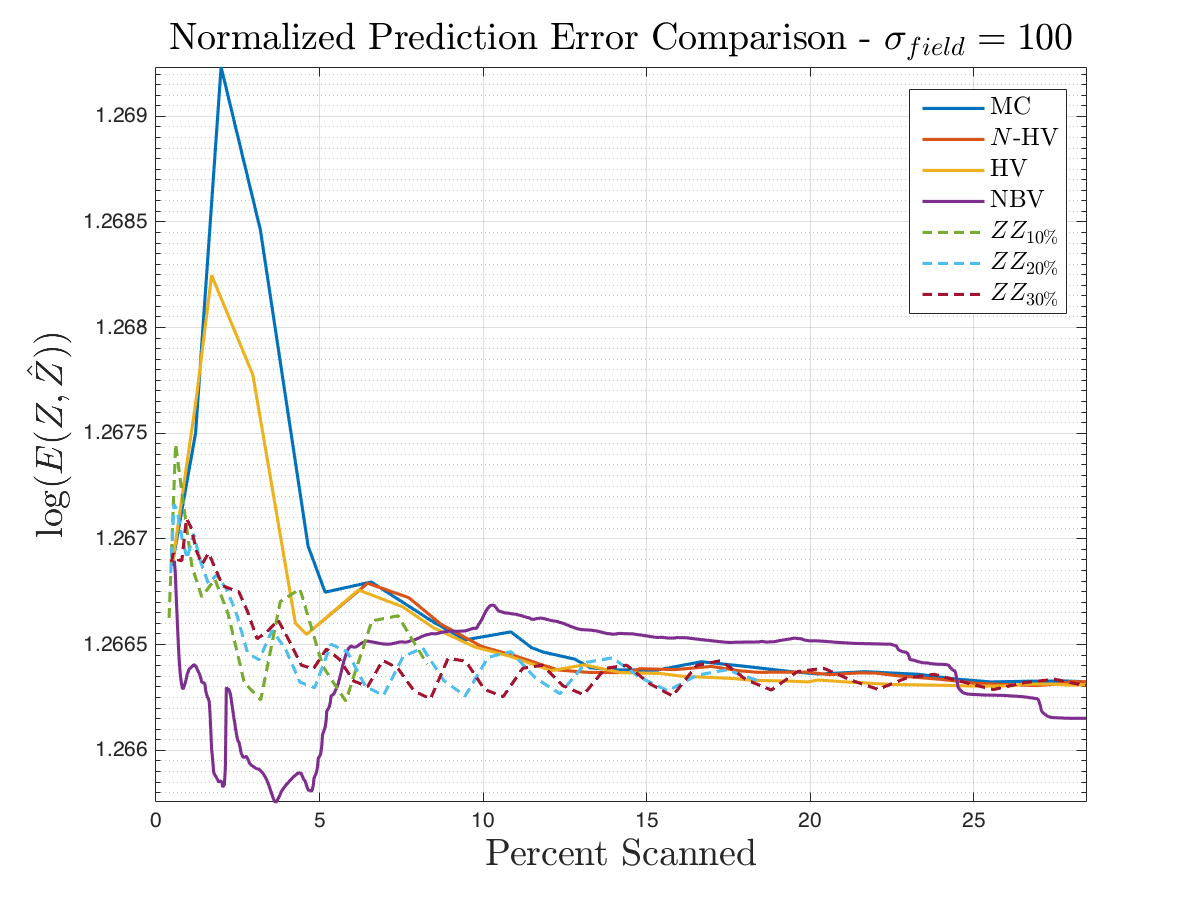
\includegraphics[width=\linewidth]{figures/normalized_errors_30p_100x100_sf_100_seed_1_app_10}
        \captionsetup{skip=0.20\baselineskip,size=footnotesize}
        \caption{Normalized prediction errors for each method.}
    \end{subfigure}%
    \\
    \begin{subfigure}[t]{0.75\textwidth}
        \centering
        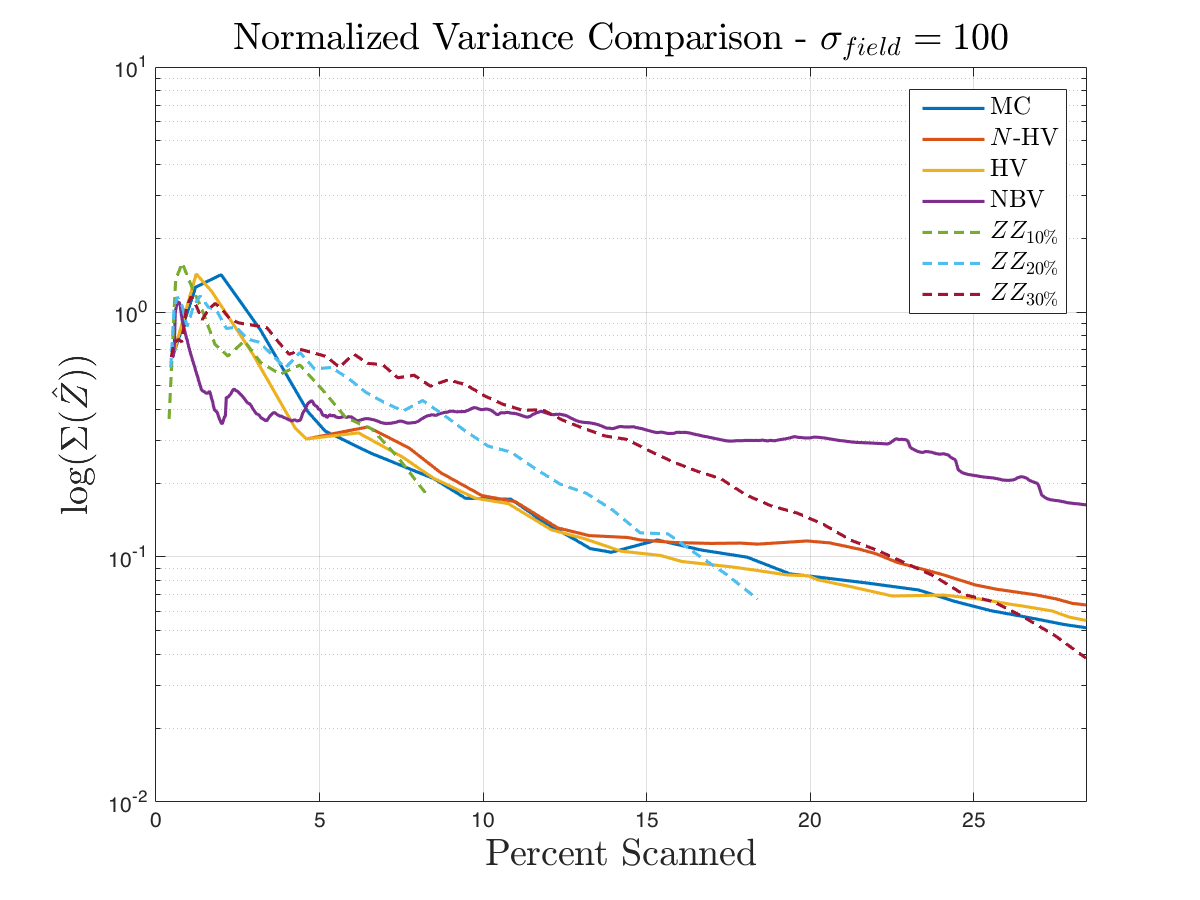
\includegraphics[width=\linewidth]{figures/normalized_variances_30p_100x100_sf_100_seed_1_app_10}
        \captionsetup{skip=0.20\baselineskip,size=footnotesize}
        \caption{Normalized prediction variances for each method.}
    \end{subfigure}%
    \captionsetup{skip=0.20\baselineskip}
    \caption{Prediction error and variances for an exploration of a field of size $100 \times 100$, $\sigma_{field} = 50$, random seed 1.}
    \label{fig:errvar50}
\end{figure}

\FloatBarrier
\clearpage

\section{Quarter Width Spatial Autocorrelation Results}
The methods will be compared on target fields generated with an autocorrelation factor, $\sigma_{field}$, that is one quarter of the field width.

\begin{figure}[htb!]
    \centering
    \begin{subfigure}[t]{0.25\textwidth}
        \centering
        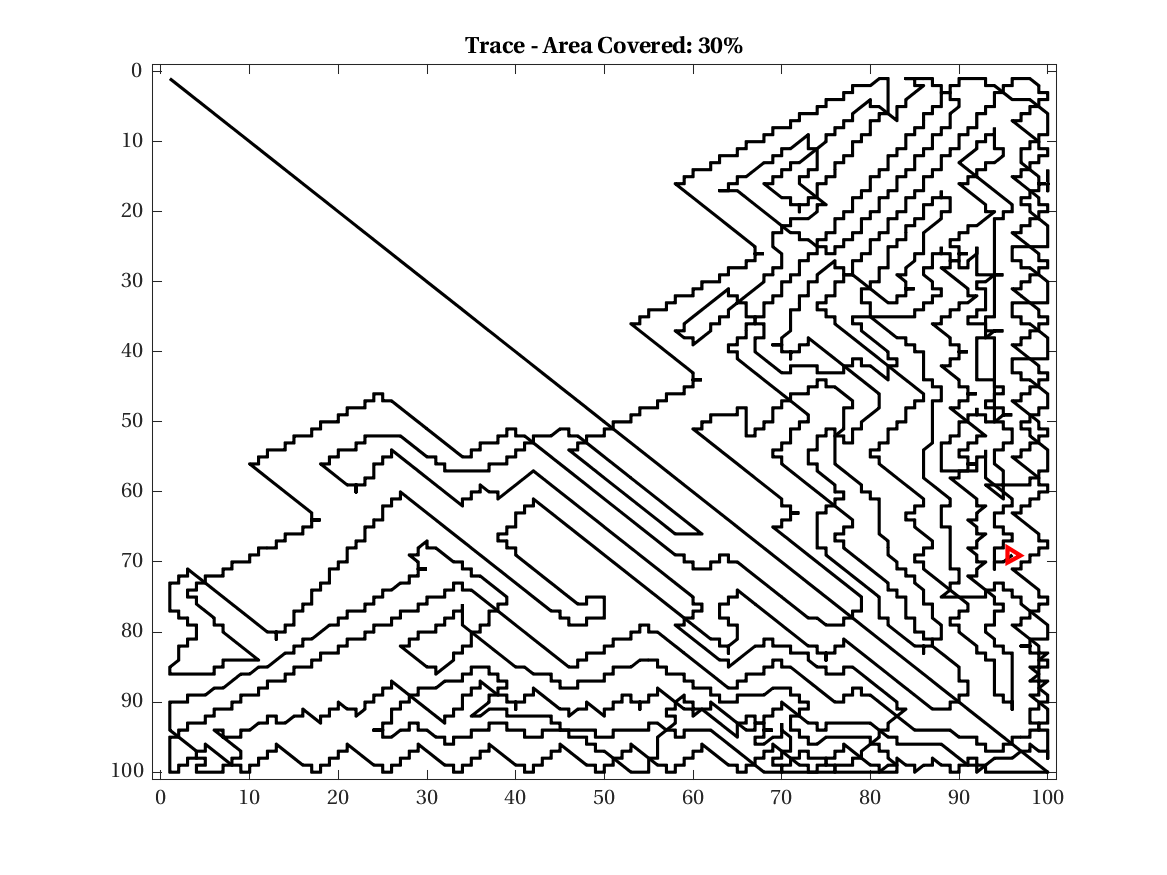
\includegraphics[width=\linewidth]{figures/path_greedy_30p_100x100_sf_25_seed_1.png}
        \captionsetup{skip=0.20\baselineskip,size=footnotesize}
        \caption{Greedy NBV}
    \end{subfigure}%
    \begin{subfigure}[t]{0.25\textwidth}
        \centering
        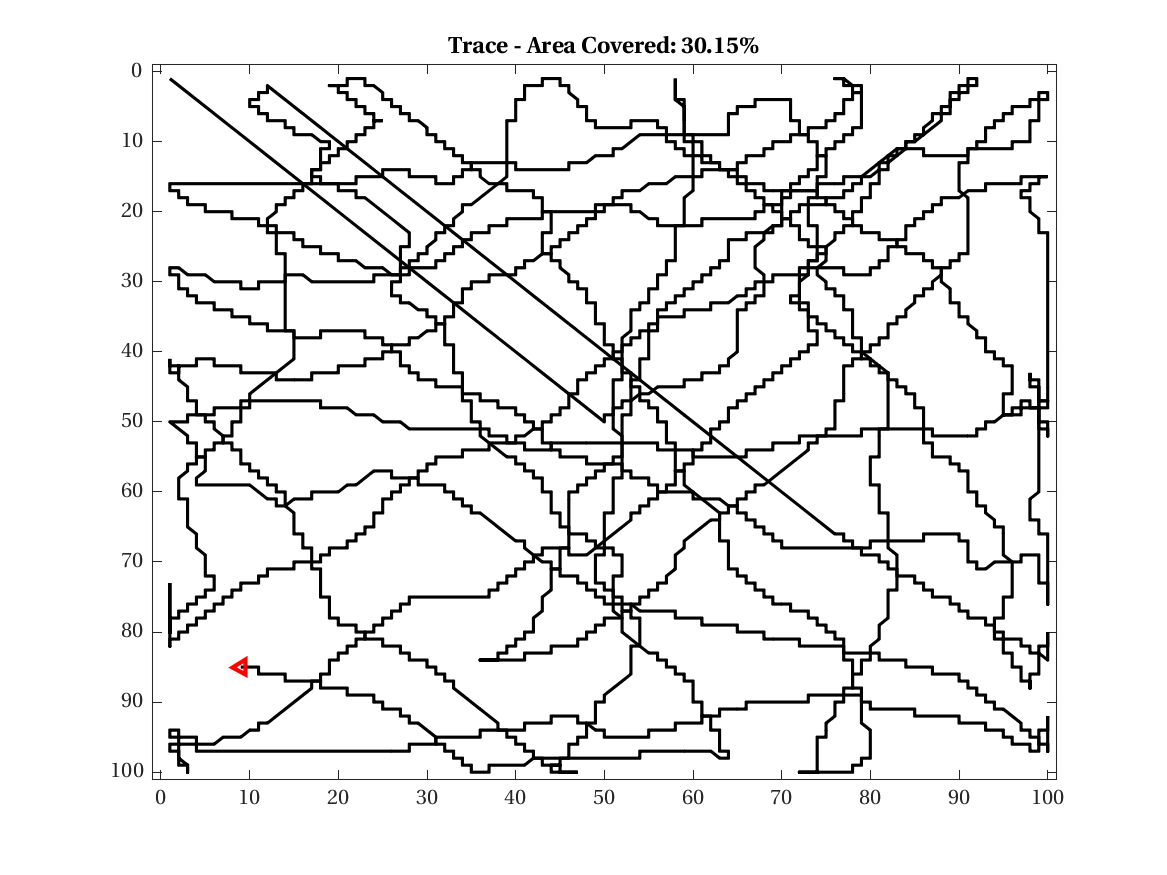
\includegraphics[width=\linewidth]{figures/path_mc_30p_100x100_sf_25_seed_1.png}
        \captionsetup{skip=0.20\baselineskip,size=footnotesize}
        \caption{MCPP}
    \end{subfigure}%
    \begin{subfigure}[t]{0.25\textwidth}
        \centering
        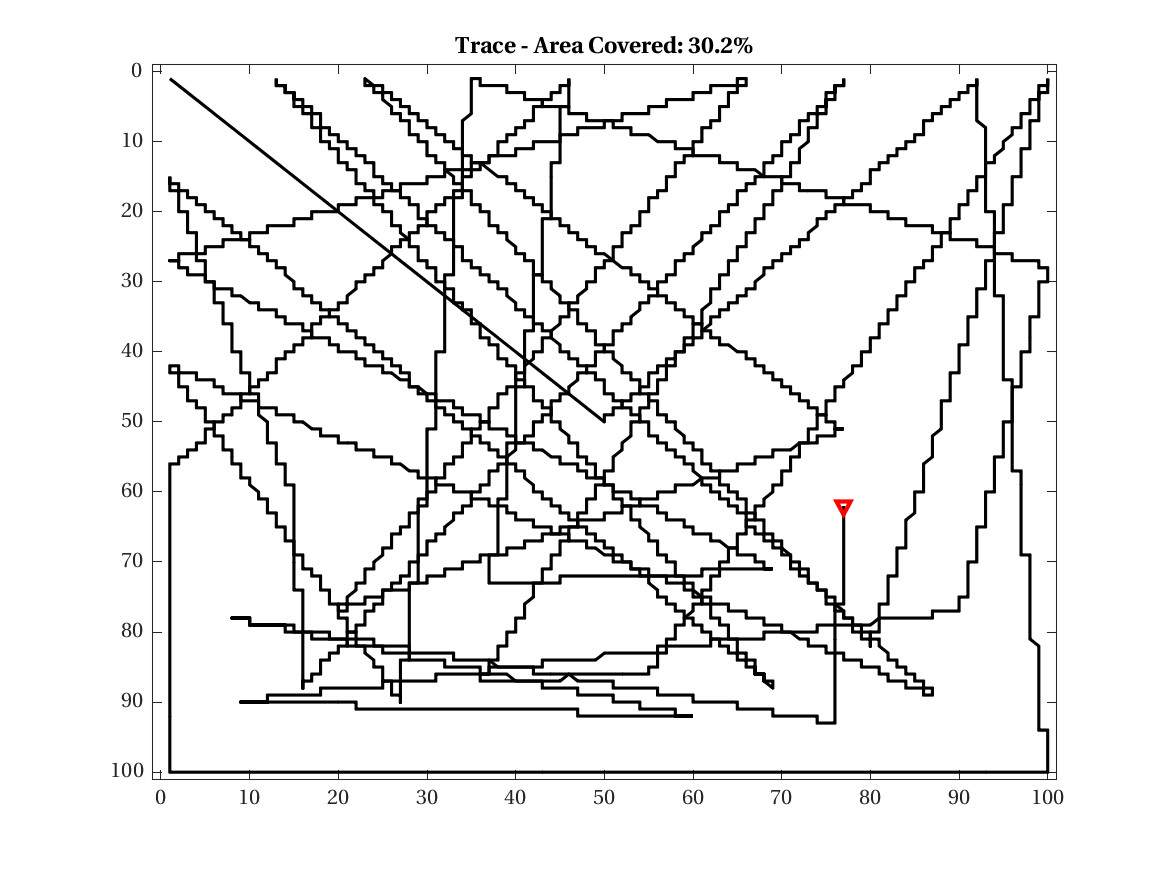
\includegraphics[width=\linewidth]{figures/path_nhv_30p_100x100_sf_25_seed_1.png}
        \captionsetup{skip=0.20\baselineskip,size=footnotesize}
        \caption{HV}
    \end{subfigure}%
    \begin{subfigure}[t]{0.25\textwidth}
        \centering
        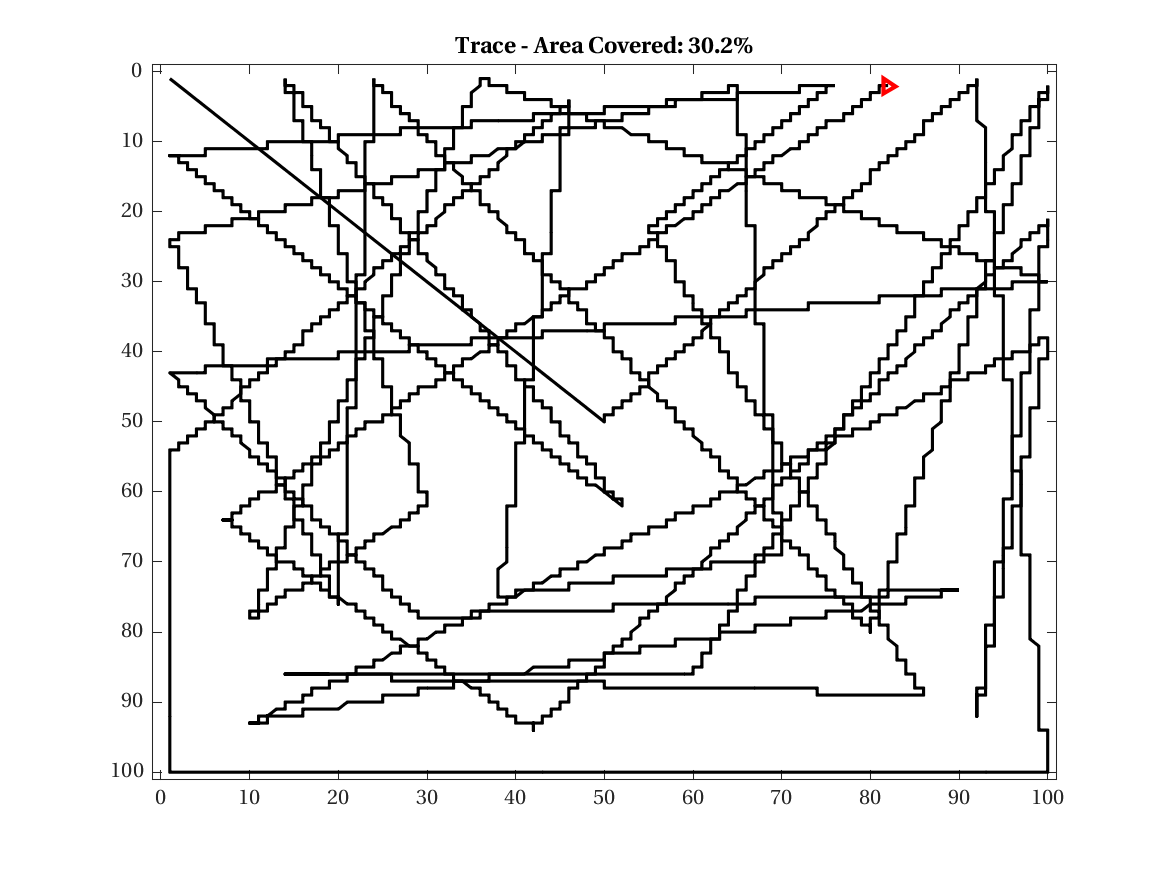
\includegraphics[width=\linewidth]{figures/path_nnhv_30p_100x100_sf_25_seed_1.png}
        \captionsetup{skip=0.20\baselineskip,size=footnotesize}
        \caption{$N$-HV}
    \end{subfigure}%
    \\
    \begin{subfigure}[t]{0.25\textwidth}
        \centering
        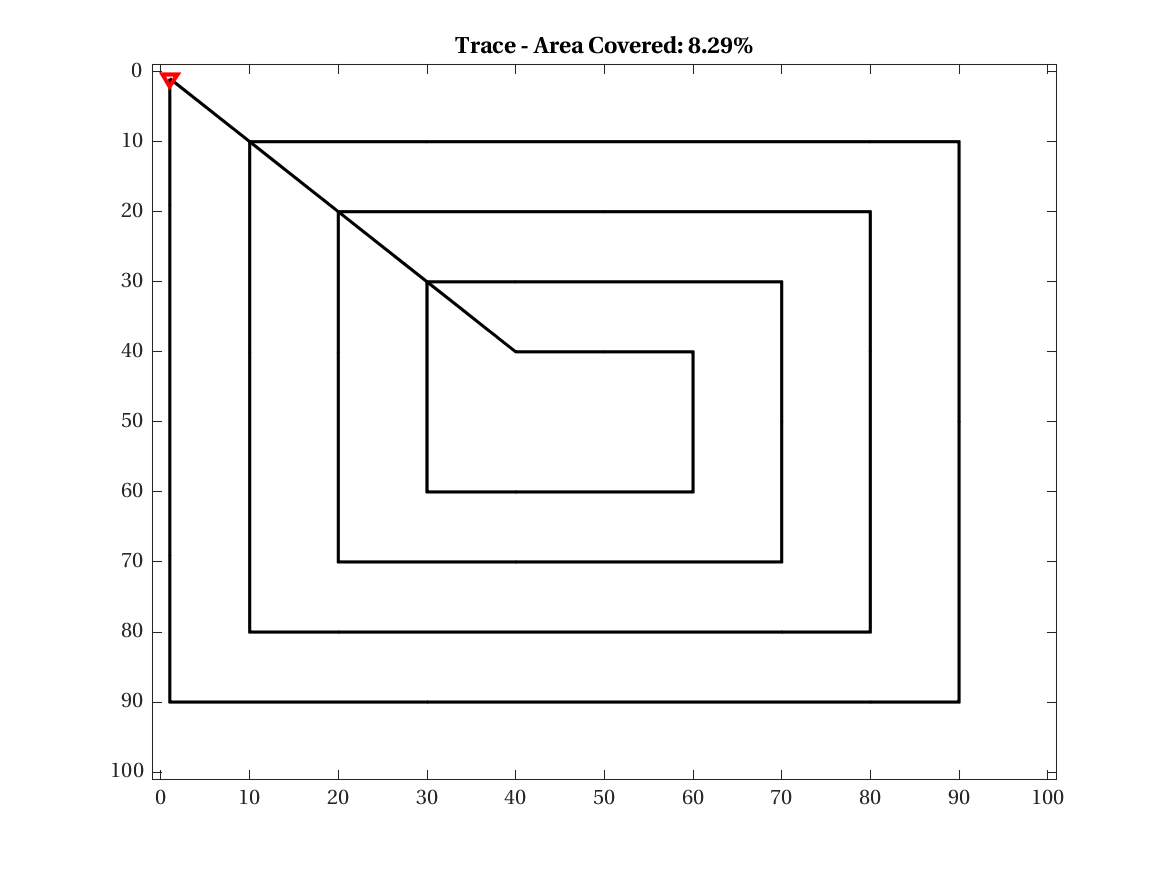
\includegraphics[width=\linewidth]{figures/path_zz_10p_100x100_sf_25_seed_1.png}
        \captionsetup{skip=0.20\baselineskip,size=footnotesize}
        \caption{$ZZ_{10}$}
    \end{subfigure}%
    \begin{subfigure}[t]{0.25\textwidth}
        \centering
        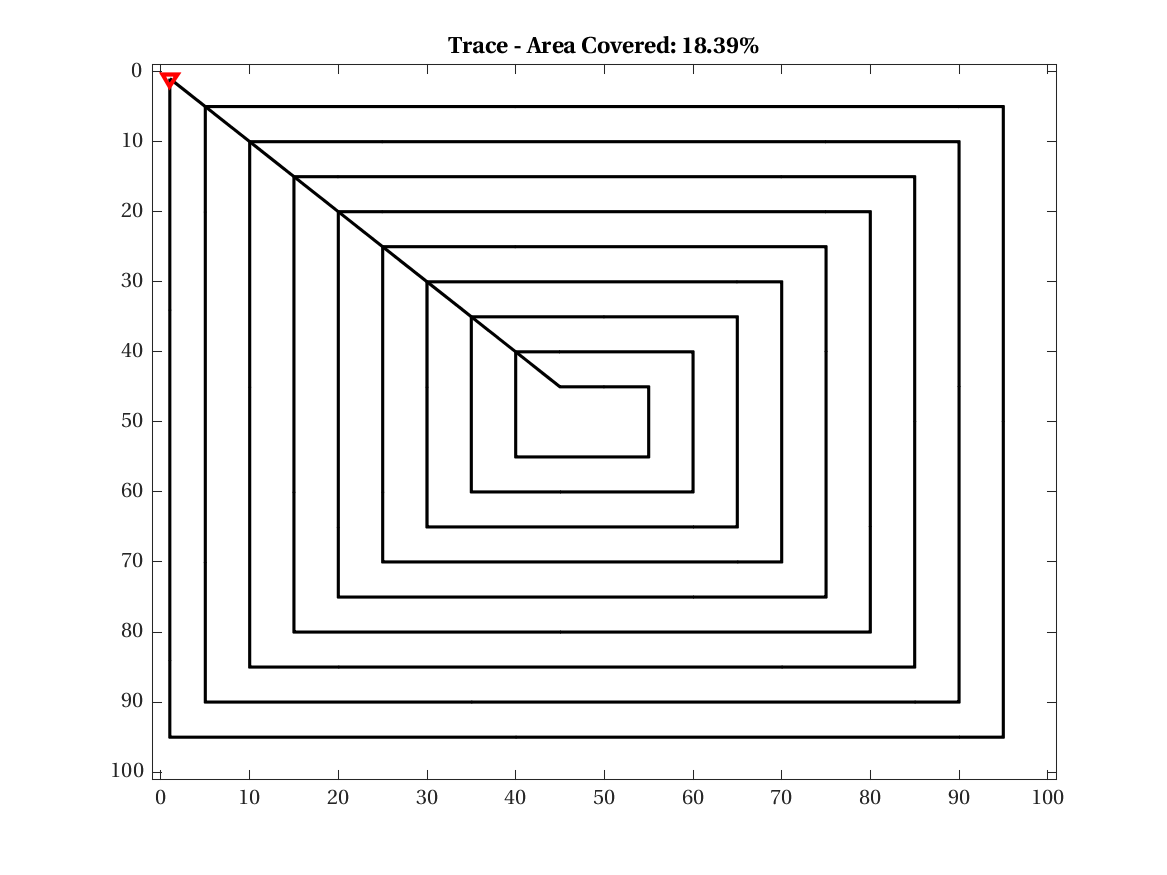
\includegraphics[width=\linewidth]{figures/path_zz_20p_100x100_sf_25_seed_1.png}
        \captionsetup{skip=0.20\baselineskip,size=footnotesize}
        \caption{$ZZ_{20}$}
    \end{subfigure}%
    \begin{subfigure}[t]{0.25\textwidth}
        \centering
        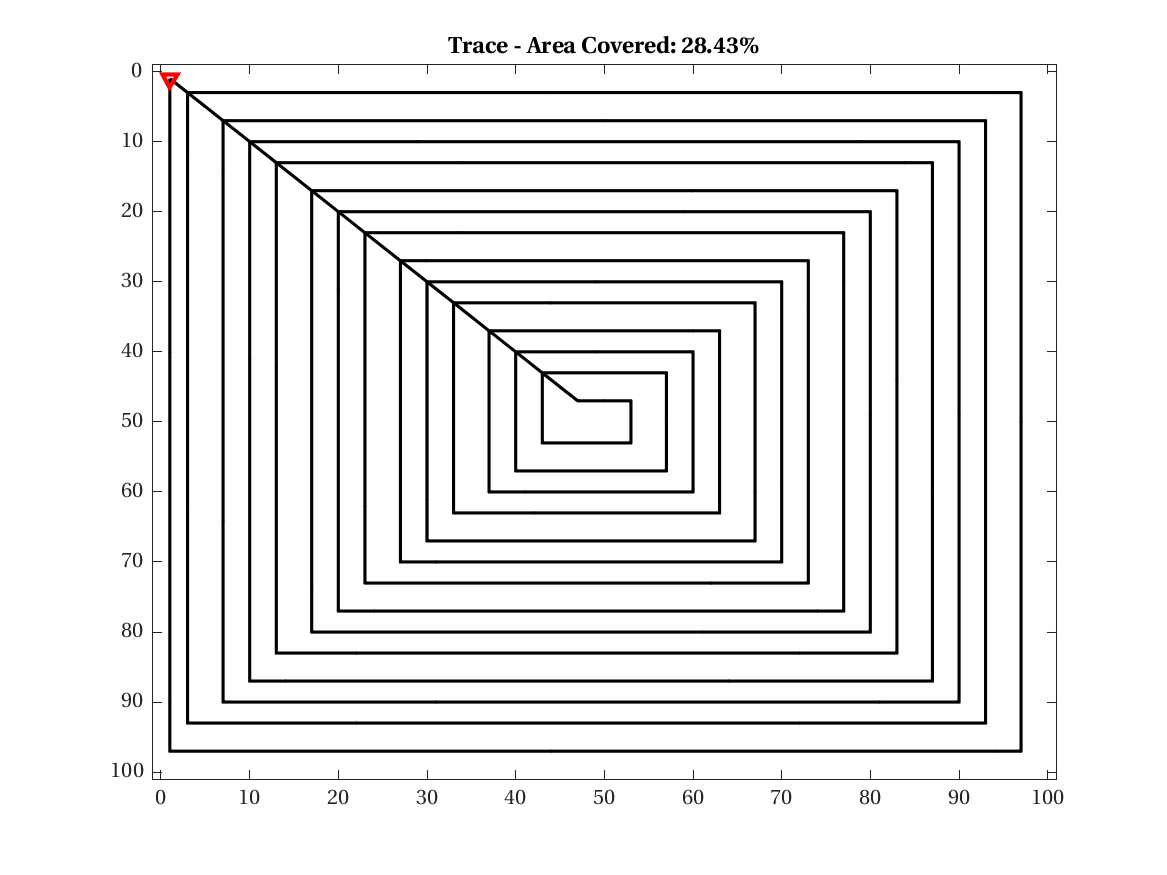
\includegraphics[width=\linewidth]{figures/path_zz_30p_100x100_sf_25_seed_1.png}
        \captionsetup{skip=0.20\baselineskip,size=footnotesize}
        \caption{$ZZ_{30}$}
    \end{subfigure}%
    \captionsetup{skip=0.20\baselineskip}
    \caption{Exploration of a field of size $100 \times 100$, $\sigma_{field} = 25$, random seed 1.}
    \label{fig:sf25}
\end{figure}

\begin{figure}[htb!]
    \centering
    \begin{subfigure}[t]{0.75\textwidth}
        \centering
        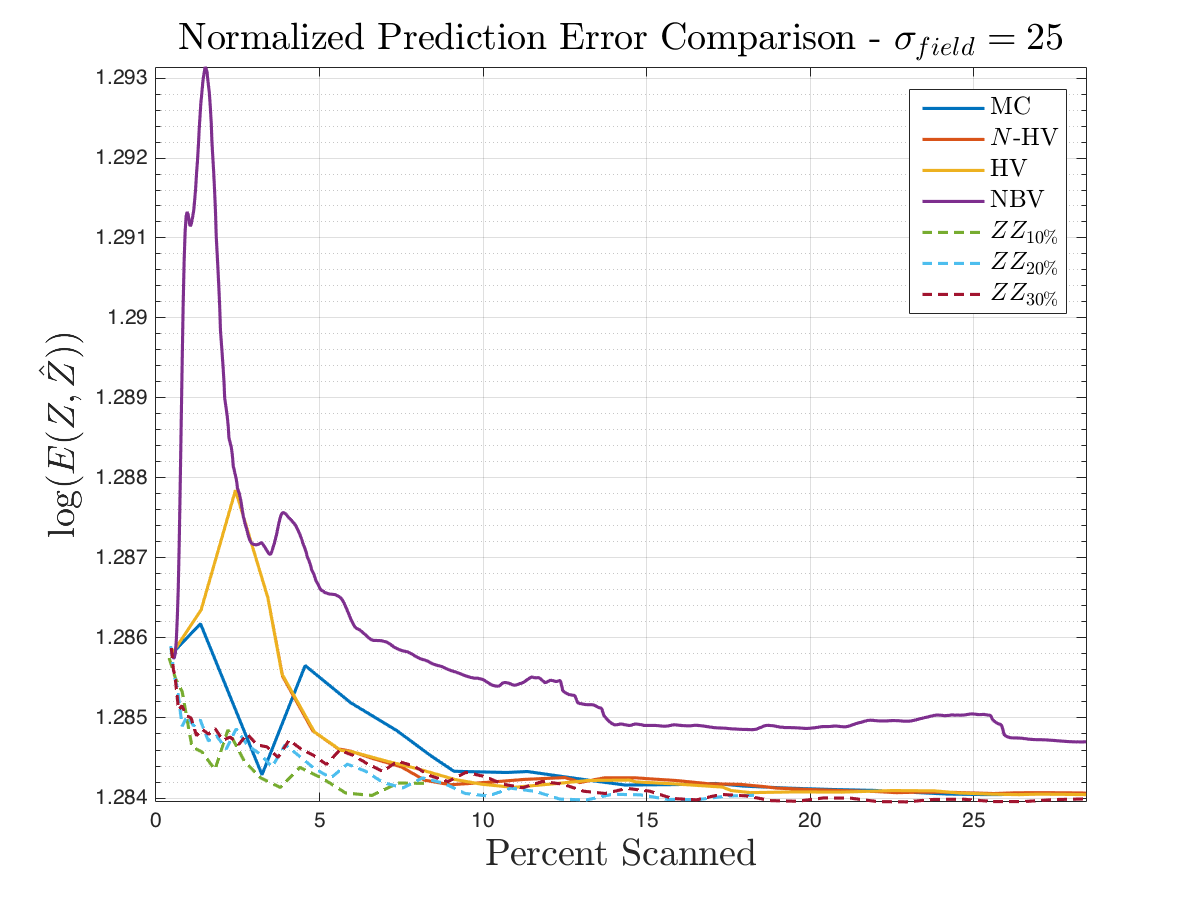
\includegraphics[width=\linewidth]{figures/normalized_errors_30p_100x100_sf_25_seed_1_app_10}
        \captionsetup{skip=0.20\baselineskip,size=footnotesize}
        \caption{Normalized prediction errors for each method.}
    \end{subfigure}%
    \\
    \begin{subfigure}[t]{0.75\textwidth}
        \centering
        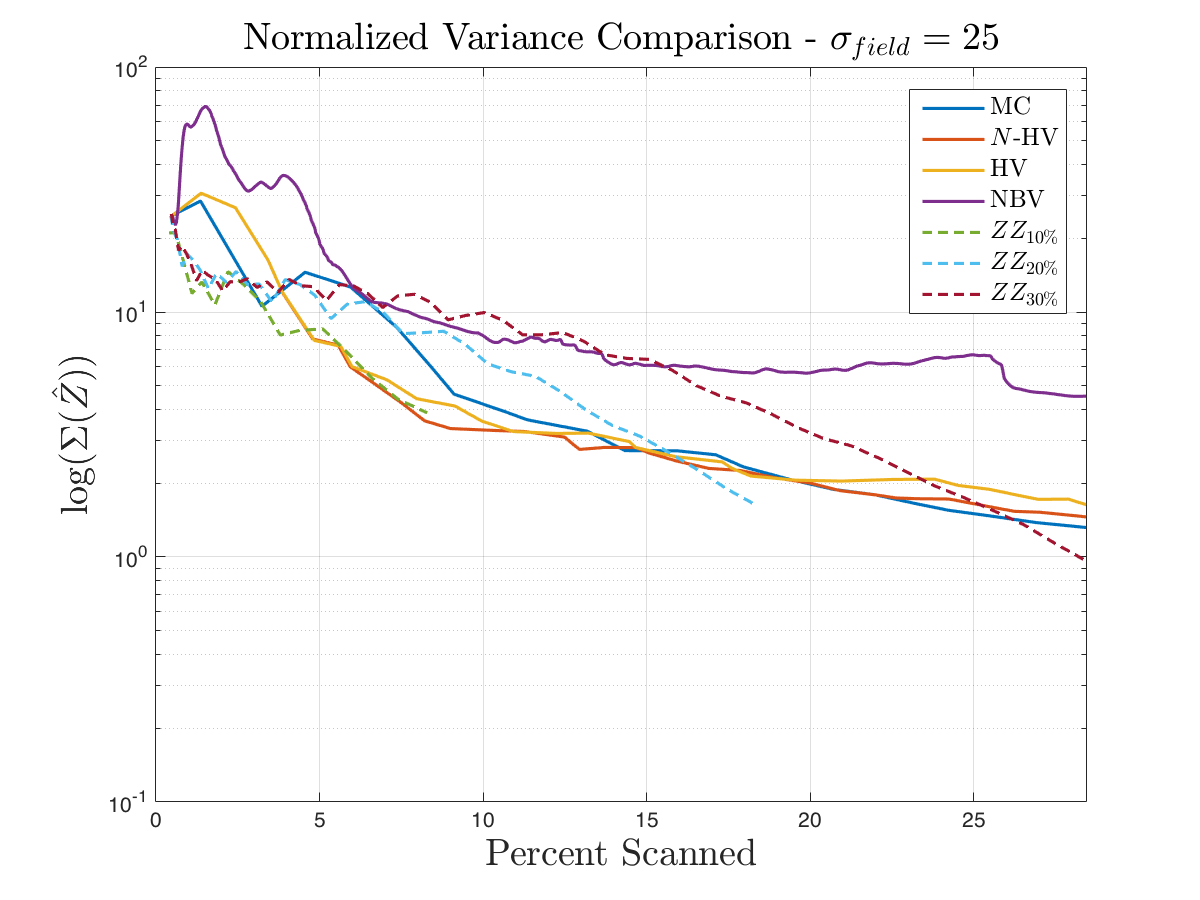
\includegraphics[width=\linewidth]{figures/normalized_variances_30p_100x100_sf_25_seed_1_app_10}
        \captionsetup{skip=0.20\baselineskip,size=footnotesize}
        \caption{Normalized prediction variances for each method.}
    \end{subfigure}%
    \captionsetup{skip=0.20\baselineskip}
    \caption{Prediction error and variances for an exploration of a field of size $100 \times 100$, $\sigma_{field} = 25$, random seed 1.}
    \label{fig:errvar25}
\end{figure}

\FloatBarrier
\clearpage

\section{Low Spatial Autocorrelation Results}
The methods will be compared on target fields generated with a low autocorrelation factor ($\sigma_{field}=1$).

\begin{figure}[htb!]
    \centering
    \begin{subfigure}[t]{0.25\textwidth}
        \centering
        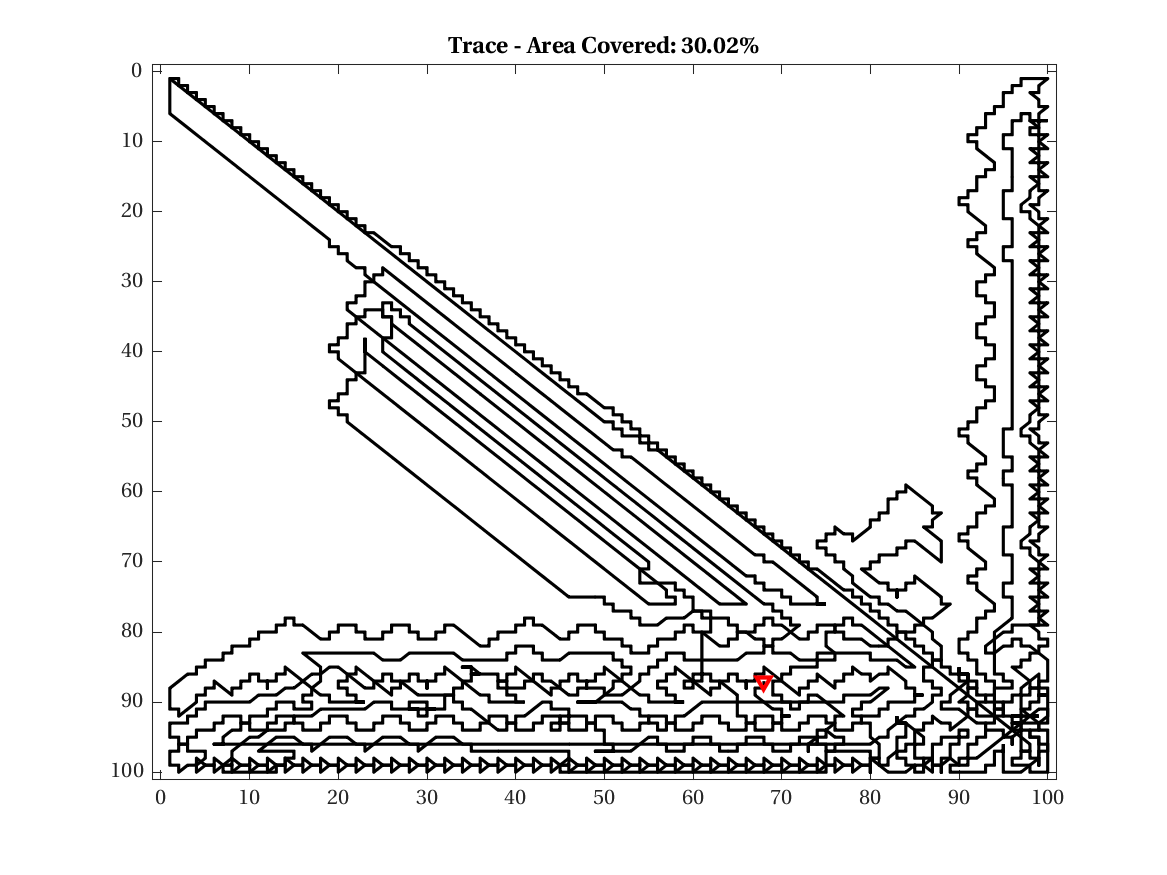
\includegraphics[width=\linewidth]{figures/path_greedy_30p_100x100_sf_1_seed_1.png}
        \captionsetup{skip=0.20\baselineskip,size=footnotesize}
        \caption{Greedy NBV}
    \end{subfigure}%
    \begin{subfigure}[t]{0.25\textwidth}
        \centering
        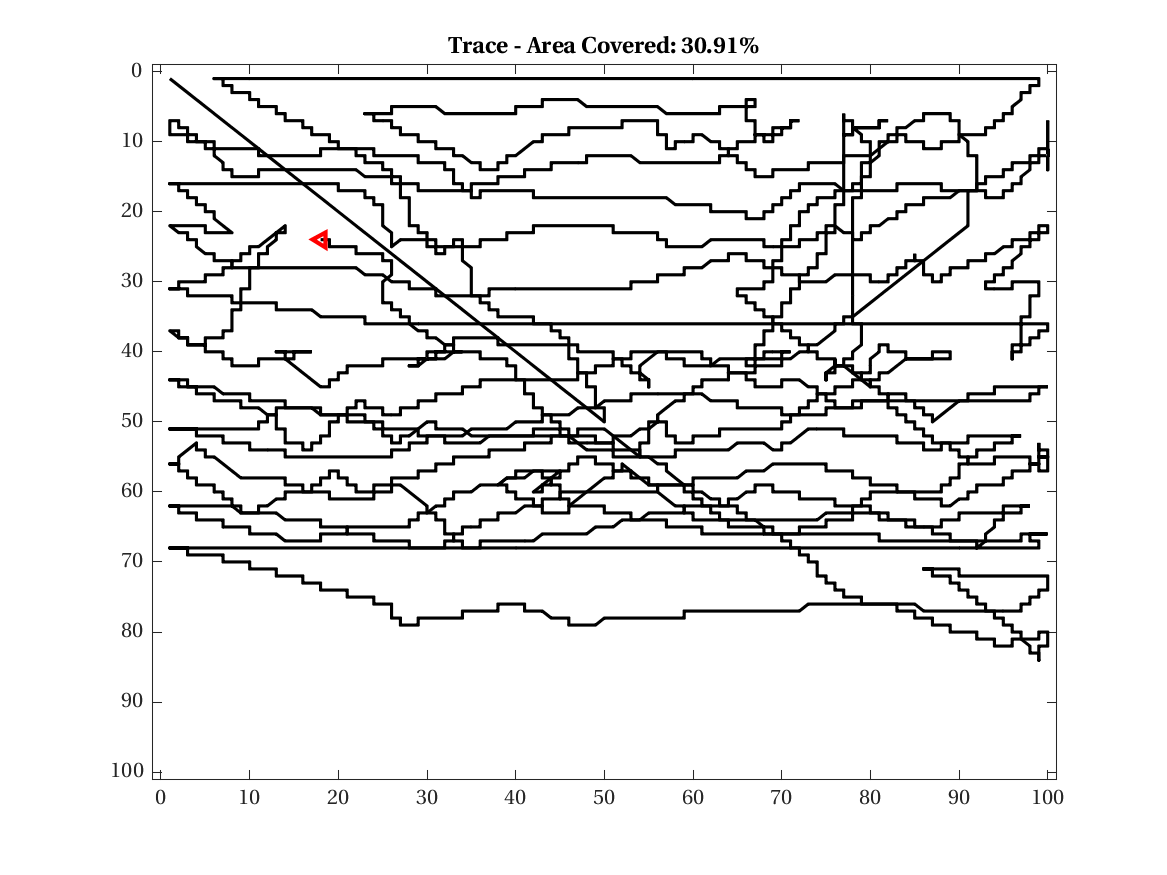
\includegraphics[width=\linewidth]{figures/path_mc_30p_100x100_sf_1_seed_1.png}
        \captionsetup{skip=0.20\baselineskip,size=footnotesize}
        \caption{MCPP}
    \end{subfigure}%
    \begin{subfigure}[t]{0.25\textwidth}
        \centering
        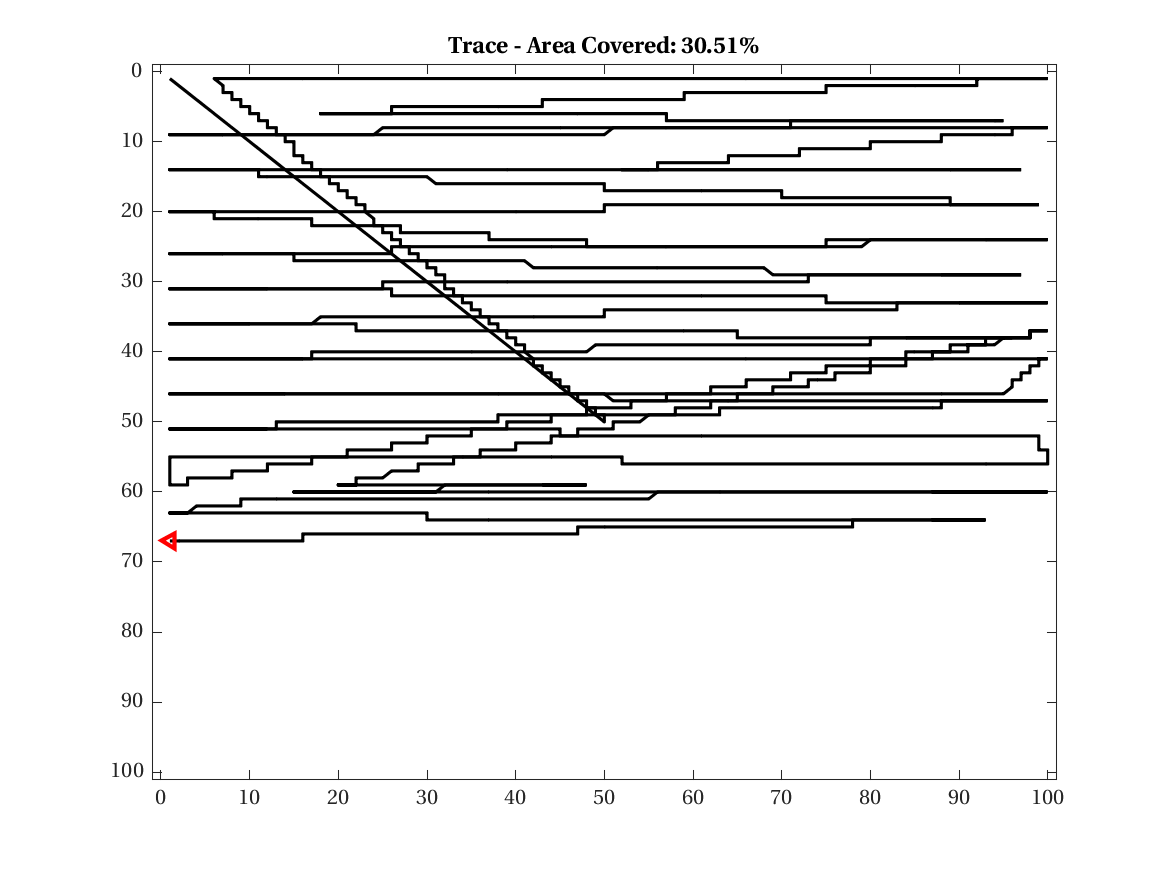
\includegraphics[width=\linewidth]{figures/path_nhv_30p_100x100_sf_1_seed_1.png}
        \captionsetup{skip=0.20\baselineskip,size=footnotesize}
        \caption{HV}
    \end{subfigure}%
    \begin{subfigure}[t]{0.25\textwidth}
        \centering
        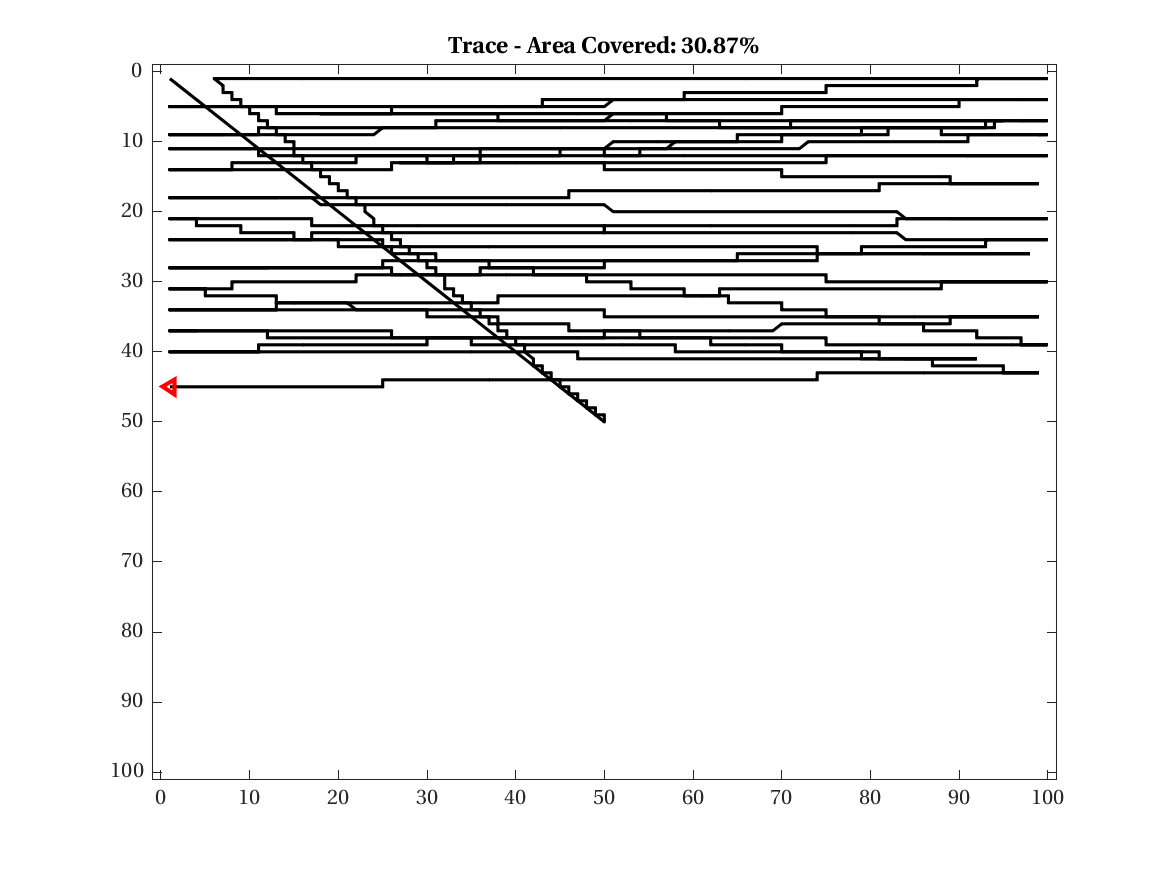
\includegraphics[width=\linewidth]{figures/path_nnhv_30p_100x100_sf_1_seed_1.png}
        \captionsetup{skip=0.20\baselineskip,size=footnotesize}
        \caption{$N$-HV}
    \end{subfigure}%
    \\
    \begin{subfigure}[t]{0.25\textwidth}
        \centering
        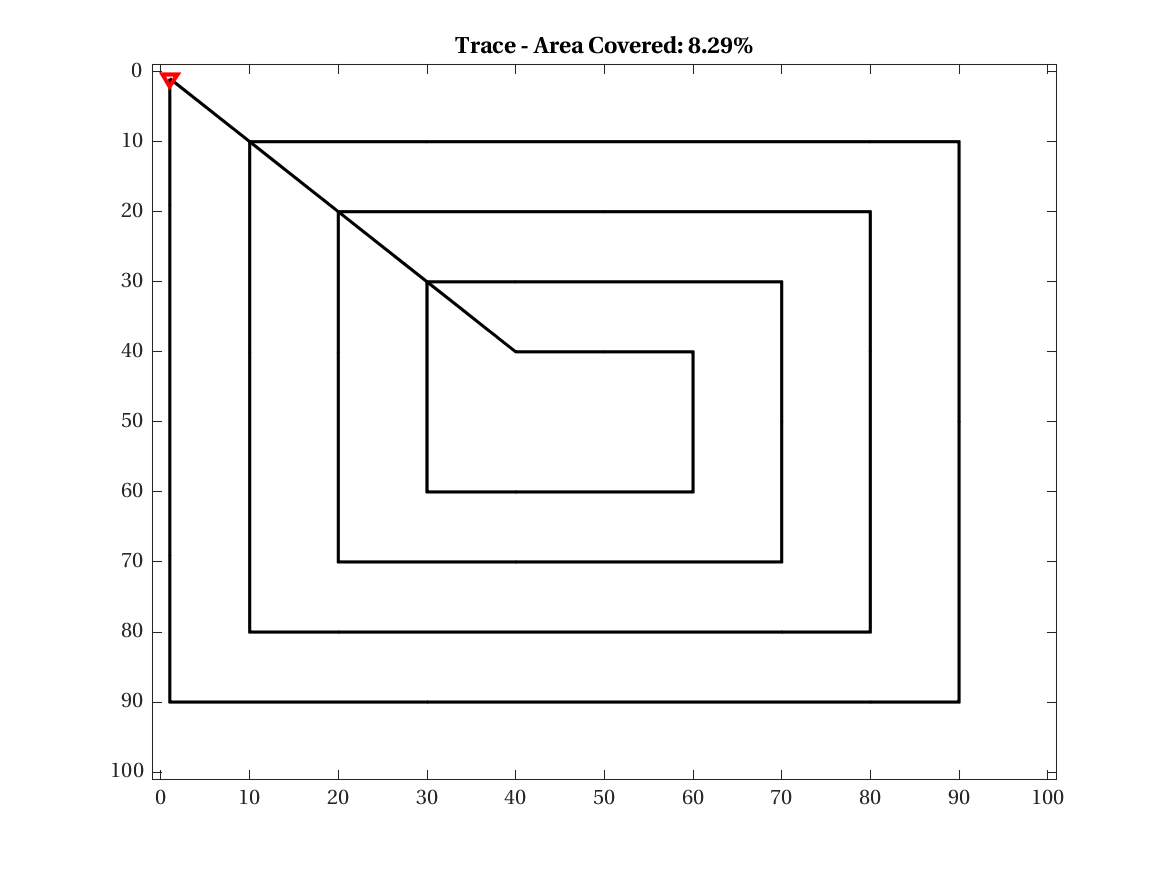
\includegraphics[width=\linewidth]{figures/path_zz_10p_100x100_sf_1_seed_1.png}
        \captionsetup{skip=0.20\baselineskip,size=footnotesize}
        \caption{$ZZ_{10}$}
    \end{subfigure}%
    \begin{subfigure}[t]{0.25\textwidth}
        \centering
        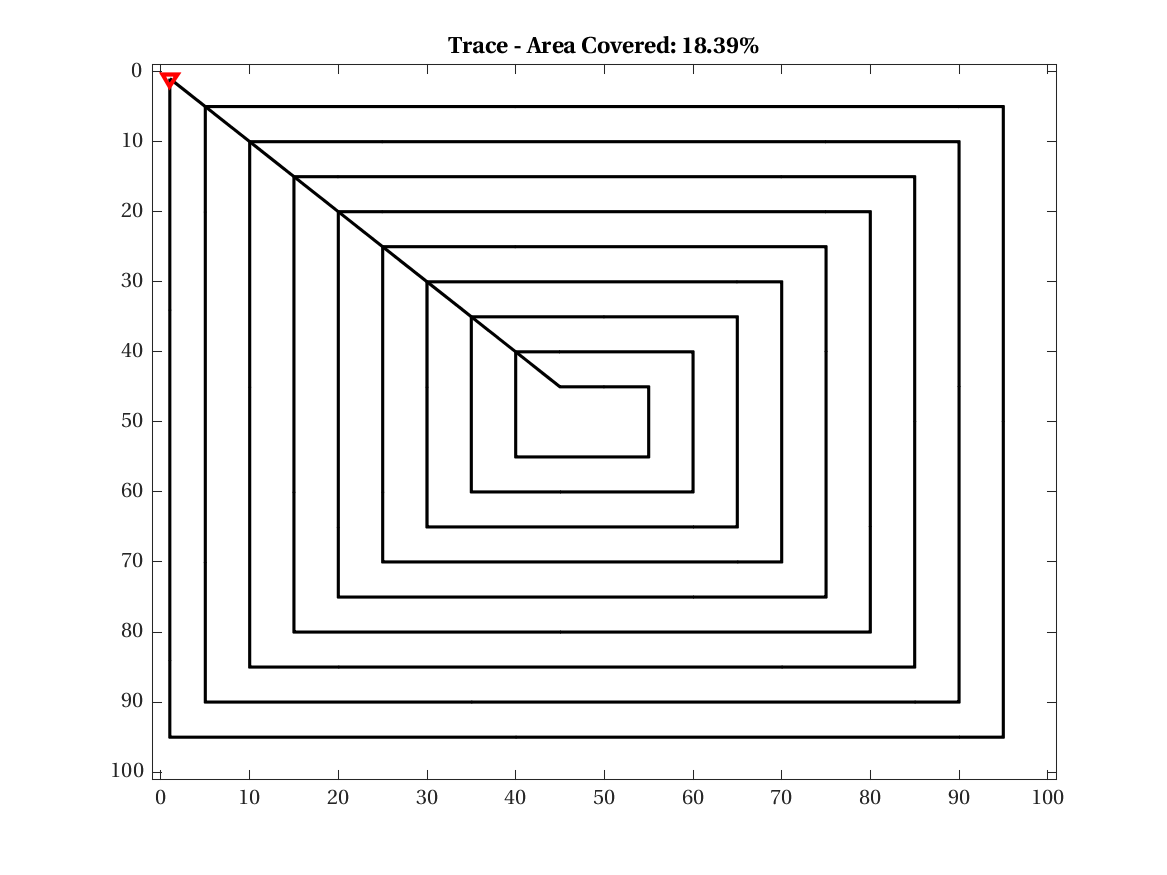
\includegraphics[width=\linewidth]{figures/path_zz_20p_100x100_sf_1_seed_1.png}
        \captionsetup{skip=0.20\baselineskip,size=footnotesize}
        \caption{$ZZ_{20}$}
    \end{subfigure}%
    \begin{subfigure}[t]{0.25\textwidth}
        \centering
        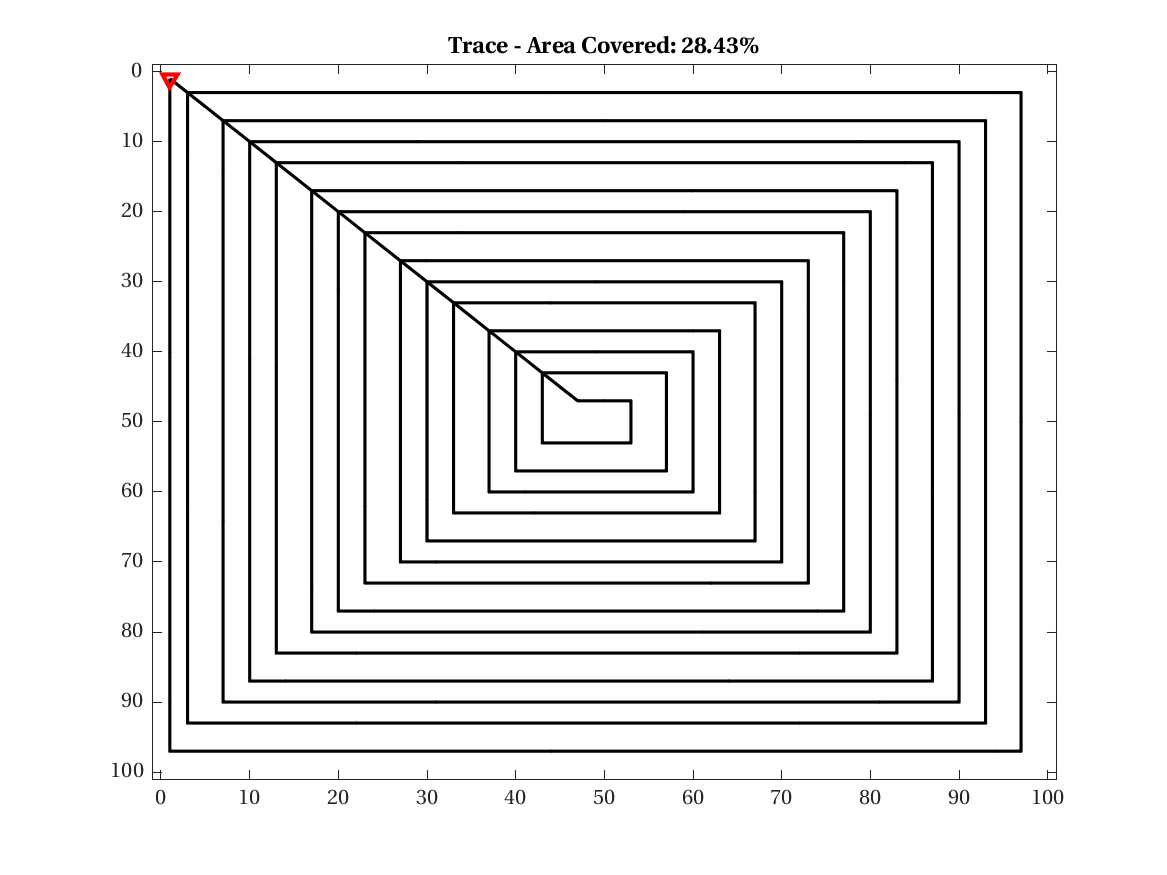
\includegraphics[width=\linewidth]{figures/path_zz_30p_100x100_sf_1_seed_1.png}
        \captionsetup{skip=0.20\baselineskip,size=footnotesize}
        \caption{$ZZ_{30}$}
    \end{subfigure}%
    \captionsetup{skip=0.20\baselineskip}
    \caption{Exploration of a field of size $100 \times 100$, $\sigma_{field} = 1$, random seed 1.}
    \label{fig:sf1}
\end{figure}

\begin{figure}[htb!]
    \centering
    \begin{subfigure}[t]{0.75\textwidth}
        \centering
        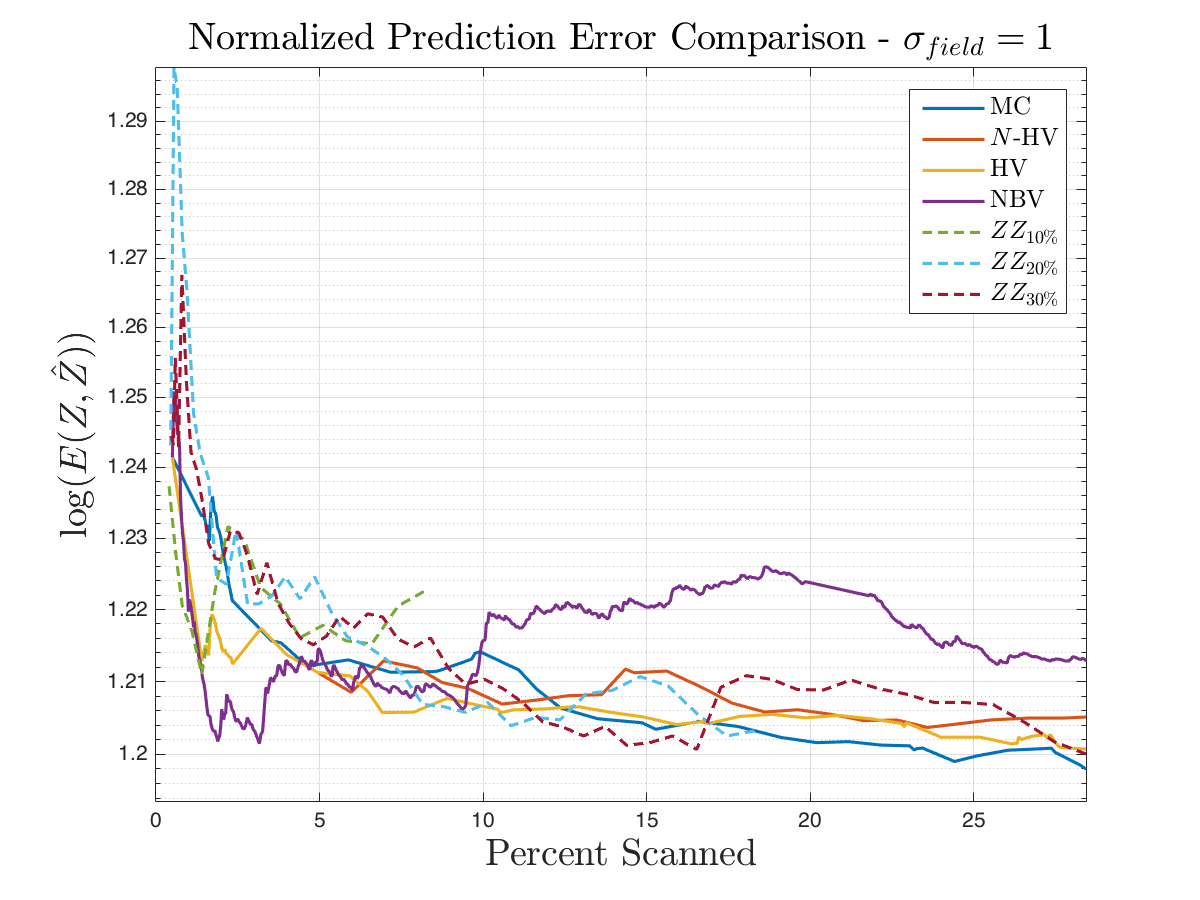
\includegraphics[width=\linewidth]{figures/normalized_errors_30p_100x100_sf_1_seed_1_app_10}
        \captionsetup{skip=0.20\baselineskip,size=footnotesize}
        \caption{Normalized prediction errors for each method.}
    \end{subfigure}%
    \\
    \begin{subfigure}[t]{0.75\textwidth}
        \centering
        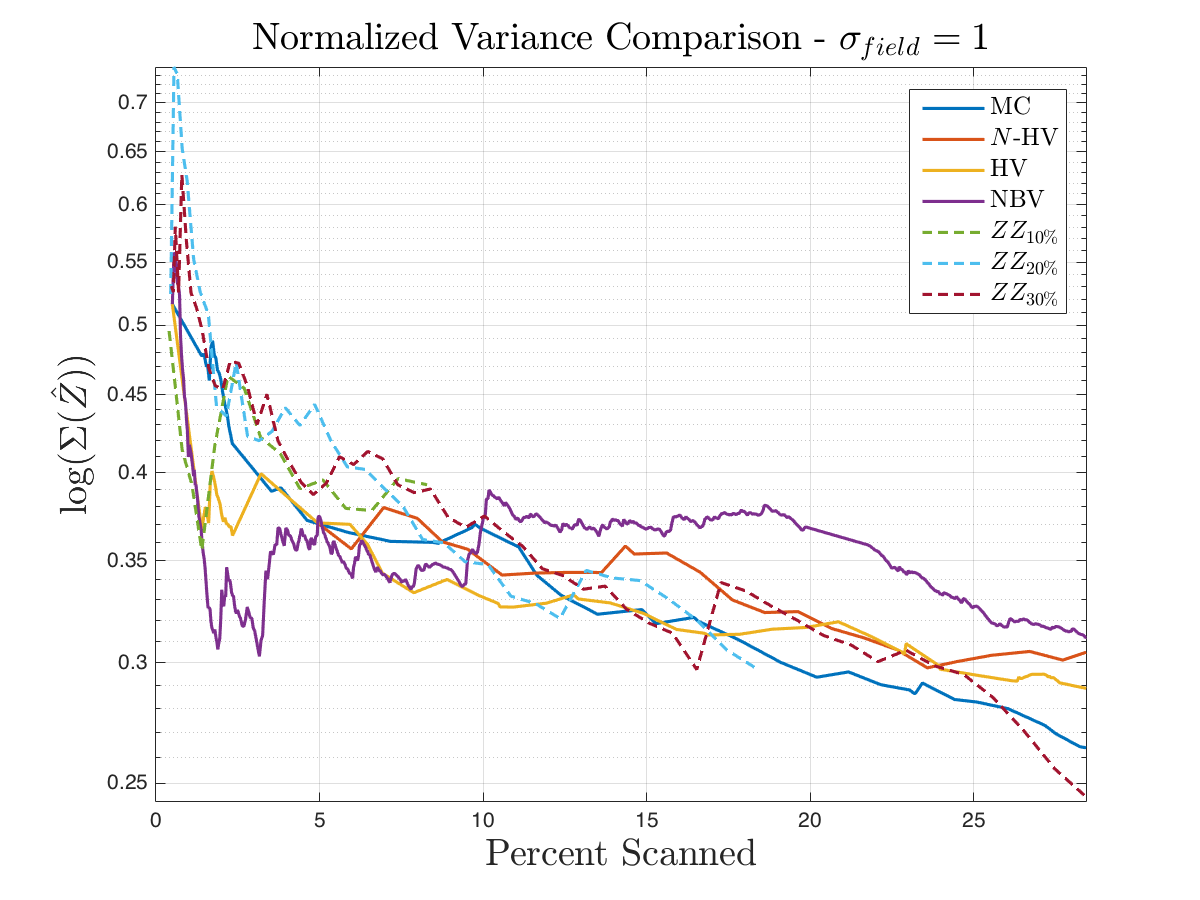
\includegraphics[width=\linewidth]{figures/normalized_variances_30p_100x100_sf_1_seed_1_app_10}
        \captionsetup{skip=0.20\baselineskip,size=footnotesize}
        \caption{Normalized prediction variances for each method.}
    \end{subfigure}%
    \captionsetup{skip=0.20\baselineskip}
    \caption{Prediction error and variances for an exploration of a field of size $100 \times 100$, $\sigma_{field} = 1$, random seed 1.}
    \label{fig:errvar1}
\end{figure}
\clearpage

\section{Comparing The Methods}
The three path planners introduced (HV, $N$-HV, MCPP) more effectively reduce prediction variance when compared to the Greedy NBV and the zig-zag methods. TODO